%% For double-blind review submission, w/o CCS and ACM Reference (max submission space)
%\documentclass[acmsmall,review]{acmart}\settopmatter{printfolios=true,printccs=false,printacmref=false}
%% For double-blind review submission, w/ CCS and ACM Reference
\documentclass[acmsmall,review,anonymous]{acmart}\settopmatter{printfolios=true}
%% For single-blind review submission, w/o CCS and ACM Reference (max submission space)
%\documentclass[acmsmall,review]{acmart}\settopmatter{printfolios=true,printccs=false,printacmref=false}
%% For single-blind review submission, w/ CCS and ACM Reference
%\documentclass[acmsmall,review]{acmart}\settopmatter{printfolios=true}
%% For final camera-ready submission, w/ required CCS and ACM Reference
%\documentclass[acmsmall]{acmart}\settopmatter{}
\usepackage{enumitem}
\usepackage{mathtools}
% \usepackage{ amssymb }
\DeclareTextFontCommand{\texttt}{\ttfamily}

%% Journal information
%% Supplied to authors by publisher for camera-ready submission;
%% use defaults for review submission.
\acmJournal{PACMPL}
\acmVolume{1}
\acmNumber{OOPSLA} % CONF = POPL or ICFP or OOPSLA
\acmArticle{1}
\acmYear{2022}
\acmMonth{1}
\acmDOI{} % \acmDOI{10.1145/nnnnnnn.nnnnnnn}
\startPage{1}

%% Copyright information
%% Supplied to authors (based on authors' rights management selection;
%% see authors.acm.org) by publisher for camera-ready submission;
%% use 'none' for review submission.
\setcopyright{none}
%\setcopyright{acmcopyright}
%\setcopyright{acmlicensed}
%\setcopyright{rightsretained}
%\copyrightyear{2018}           %% If different from \acmYear

%% Bibliography style
\bibliographystyle{ACM-Reference-Format}
%% Citation style
%% Note: author/year citations are required for papers published as an
%% issue of PACMPL.
\citestyle{acmauthoryear}   %% For author/year citations


%%%%%%%%%%%%%%%%%%%%%%%%%%%%%%%%%%%%%%%%%%%%%%%%%%%%%%%%%%%%%%%%%%%%%%
%% Note: Authors migrating a paper from PACMPL format to traditional
%% SIGPLAN proceedings format must update the '\documentclass' and
%% topmatter commands above; see 'acmart-sigplanproc-template.tex'.
%%%%%%%%%%%%%%%%%%%%%%%%%%%%%%%%%%%%%%%%%%%%%%%%%%%%%%%%%%%%%%%%%%%%%%


%% Some recommended packages.
\usepackage{booktabs}   %% For formal tables:
                        %% http://ctan.org/pkg/booktabs
\usepackage{subcaption} %% For complex figures with subfigures/subcaptions
                        %% http://ctan.org/pkg/subcaption
 \usepackage{ stmaryrd }                       

\usepackage{relsize}
\usepackage{mathpartir}
\usepackage{amsmath}
\usepackage{amsthm}
\usepackage{listings}
\usepackage{xspace}
\usepackage{definitions}
\usepackage{multirow,bigdelim}
\usepackage{pbox}
\usepackage{courier}
\usepackage{soul}
\usepackage{centernot}

\newcommand\multibrace[3]{\rdelim\}{#1}{3mm}[\pbox{#2}{#3}]}

\definecolor{ferngreen}{rgb}{0.31, 0.47, 0.26}
\newcommand{\kjx}[1]{{\color{ferngreen}{(KJX: #1)}}}
\newcommand{\scd}[1]{{\color{blue}{#1}}}
%\newcommand{\sdN}[1]{{\color{dkgreen}{#1}}}
%\newcommand{\jm}[1]{{\color{magenta}{JM: #1}}}
\newcommand{\sdcomment}[1]{{\ensuremath{\blacksquare}}\footnote{\color{dkgreen}{SD: #1}}}
\newcommand{\secomment}[1]{{\ensuremath{\blacksquare}}\footnote{\se{#1}}}
\newcommand{\jncomment}[1]{{\ensuremath{\blacksquare}}\footnote{\kjx{#1}}}

\newcommand{\sd}[1]{{\color{blue}{#1}}}
 \newcommand{\tobyM}[1]{#1} %[1]{{\color{purple}{Toby: #1}}}
\newcommand{\se}[1]{{\color{green}{#1}}}
\definecolor{amber}{rgb}{1.0, 0.75, 0.0}
\definecolor{amethyst}{rgb}{0.6, 0.4, 0.8}

\newcommand{\ponders}[3]{\marginpar{\tiny\itshape\raggedright\textcolor{#2}{\textbf{#1:} #3}}\ignorespaces}
\marginparwidth=1.6cm \marginparsep=0cm
\newcommand{\TODO}[1]{} % {{\color{red}#1}}
\newcommand{\sophia}[1]{{\color{blue}#1}}
\newcommand{\toby}[1]{} % {\ponders{Toby}{purple}{#1}}
\newcommand{\susan}[2][]{\ponders{Susan}{brown}{#1} \textcolor{brown}{#2}\xspace}
\newcommand{\james}[1]{\ponders{James}{orange}{#1}}
\newcommand{\jm}[2][]{\ponders{Julian}{magenta}{#1} \textcolor{magenta}{#2}\xspace}
\newcommand{\mrr}[2][]{\ponders{Matthew Ross}{offblue}{{#1}} \textcolor{offblue}{{#2}}\xspace}
\newcommand{\sdr}[2][]{\ponders{SD:}{blue}{#1} \textcolor{blue}{#2}\xspace}
\newcommand{\sdNr}[2][]{\ponders{SD:}{amber}{#1} \textcolor{amethyst}{#2}\xspace}
\newcommand{\sdN}[1]{{\color{teal}{#1}}}
\newcommand{\mrrz}[1]{\textcolor{offblue}{{#1}}\xspace}
\newcommand{\Mrr}[2][]{\ponders{Matthew Ross}{teal}{{#1}} \textcolor{teal}{{#2}}\xspace}
\newcommand{\Mrrz}[1]{\textcolor{teal}{{#1}}\xspace}
\newcommand{\julian}[1]{\textcolor{green}{#1}\xspace}
\newcommand{\sdM}[1]{\textcolor{amethyst}#1\xspace}

\newcommand{\sophiaPonder}[2][]{\ponders{Sophia}{blue}{#1} \textcolor{blue}{#2}\xspace}
\renewcommand{\sophia}[2][]

\newcommand{\sdfootnote}[1]{\footnote{#1}}



\begin{document}

%% Title information
%\title[Specification and Proof of Necessary Conditions]{Specification
%and Proof of Necessary Conditions}         %% [Short Title] is
%optional;
%\title{Necessity Specifications are Necessary}
\title{Object Capabilities as Guards -- Current Questions}
\subtitle{Notes for internal Discussion} 
% \title{\Nec Specifications are Necessary for Robustness}

                                        %% when present, will be used in
                                        %% header instead of Full Title.
%\titlenote{with title note}             %% \titlenote is optional;
                                        %% can be repeated if necessary;
                                        %% contents suppressed with 'anonymous'
%\subtitle{Subtitle}                     %% \subtitle is optional
%\subtitlenote{with subtitle note}       %% \subtitlenote is optional;
                                        %% can be repeated if necessary;
                                        %% contents suppressed with 'anonymous'


%% Author information
%% Contents and number of authors suppressed with 'anonymous'.
%% Each author should be introduced by \author, followed by
%% \authornote (optional), \orcid (optional), \affiliation, and
%% \email.
%% An author may have multiple affiliations and/or emails; repeat the
%% appropriate command.
%% Many elements are not rendered, but should be provided for metadata
%% extraction tools.


%% Author with two affiliations and emails.
\author{Julian Mackay}
%\authornote{with author2 note}          %% \authornote is optional;
                                        %% can be repeated if necessary
\orcid{0000-0003-3098-3901}             %% \orcid is optional
\affiliation{
  %\position{Position2a}
  %\department{Engineering and Computer Science}             %% \department is recommended
  \institution{Victoria University of Wellington}           %% \institution is required
  %\streetaddress{Street2a Address2a}
  %\city{City2a}
  %\state{State2a}
  %\postcode{Post-Code2a}
  \country{New Zealand}                   %% \country is recommended
}
\email{julian.mackay@ecs.vuw.ac.nz}         %% \email is recommended

%% Author with single affiliation.
\author{Sophia Drossopoulou}
%\authornote{with author1 note}          %% \authornote is optional;
                                        %% can be repeated if necessary
\orcid{0000-0002-1993-1142}             %% \orcid is optional
\affiliation{
  %\position{Position1}
  %\department{Department1}              %% \department is recommended
  \institution{Imperial College London}            %% \institution is required
  %\streetaddress{Street1 Address1}
  %\city{City1}
  %\state{State1}
  %\postcode{Post-Code1}
  \country{United Kingdom}                    %% \country is recommended
}
\email{scd@imperial.ac.uk}          %% \email is recommended

\author{James Noble}
%\authornote{with author2 note}          %% \authornote is optional;
                                        %% can be repeated if necessary
\orcid{0000-0001-9036-5692}             %% \orcid is optional
\affiliation{
  %\position{Position2a}
  %\department{Department2a}             %% \department is recommended
  \institution{Creative Research \& Programming}           %% \institution is required
  \streetaddress{5 Fernlea Ave, Darkest Karori}
  \city{Wellington}
  %\state{State2a}
  \postcode{6012}
  \country{New Zealand}                   %% \country is recommended
}
\email{kjx@acm.org}         %% \email is recommended


\author{Susan Eisenbach}
%\authornote{with author2 note}          %% \authornote is optional;
                                        %% can be repeated if necessary
\orcid{0000-0001-9072-6689}             %% \orcid is optional
\affiliation{
  %\position{Position2a}
  %\department{}             %% \department is recommended
  \institution{Imperial College London}           %% \institution is required
  %\streetaddress{Street2a Address2a}
  %\city{City2a}
  %\state{State2a}
  %\postcode{Post-Code2a}
  \country{United Kingdom}                   %% \country is recommended
}
\email{susan@imperial.ac.uk}         %% \email is recommended



%% Abstract
 \begin{abstract}
Here the questions and worries SD had in the last 2-3 weeks. 
Luckily, after writing the current note for the discussion, SD now believes that none of these worries are valid.  :-)
SD hopes that you will agree,
This document also poses some questions of taste.
 
 \end{abstract} 
 % environment must come
%% before \maketitle command

 
  

%% 2012 ACM Computing Classification System (CSS) concepts
%% Generate at 'http://dl.acm.org/ccs/ccs.cfm'.
\begin{CCSXML}
<ccs2012>
<concept>
<concept_id>10011007.10011006.10011008</concept_id>
<concept_desc>Software and its engineering~General programming languages</concept_desc>
<concept_significance>500</concept_significance>
</concept>
<concept>
<concept_id>10003456.10003457.10003521.10003525</concept_id>
<concept_desc>Social and professional topics~History of programming languages</concept_desc>
<concept_significance>300</concept_significance>
</concept>
</ccs2012>
\end{CCSXML}

\ccsdesc[500]{Software and its engineering~General programming languages}
%% End of generated code


%% Keywords
%% comma separated list
%%%%%%%%%%%%%%%%%%%%%\keywords{keyword1, keyword2, keyword3}  %% \keywords are mandatory in final camera-ready submission



%% Note: \maketitle command must come after title commands, author
%% commands, abstract environment, Computing Classification System
%% environment and commands, and keywords command.




\maketitle 

 \newcommand{\balance}{\prg{bal}}
\newcommand{\password}{\prg{pwd}}
\newcommand{\myAccount}{\prg{accnt}}

\section{Questions arising from "deeper" mofifications of the heap}

 So far, we have considered pretty "flat" examples, where consider  at most one field read. Consider now a module with \prg{Account}s and\prg{Shop}s as below

\begin{lstlisting}[mathescape=true, language=Chainmail, frame=lines]
module $M_{as}$        
  class Password
  
  class Account
    ... as in $\ModC$
    
   class Shop
       field acc: Account
       
       method swap(a:Account)
          this.acc = a
    
\end{lstlisting}
%
  
We use the notation ${\inside{x}}$ to say that $x$ is protected. Assume that we want $M_{as}$   to satisfy

 \begin{tabular}{lcll}
 $S_{as}$   & $\triangleq$   &  $\TwoStatesQ {\prg{s}:\prg{Shop}}  {\inside{\prg{s.acc.pwd}}}  {\inside{\prg{s.acc.pwd}}}$
 \end{tabular}
  
\subsection{Changing footprints}  

Note that the ``footprint'' of $S_{as}$ in the pre-state may be different than that on the post-state. For example, if we have a shop a in the original configuration below,  and execute \prg{s.swap(4)}. then we obtain the configuration to the right. In the original configuration the footprint of \prg{5.acc.pwd} consists of $\{ 1. 2, 3\}$, but in the second configuration it consists of $\{ 1. 4, 5\}$
  
\begin{figure}[htb]
\begin{tabular}{|c|c|}
\hline \\
\resizebox{4.5cm}{!}{
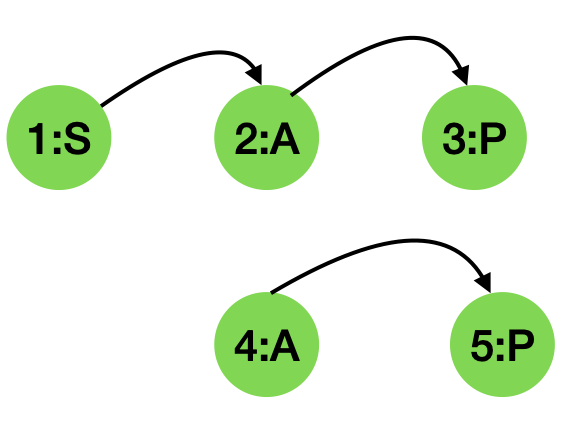
\includegraphics[width=\linewidth]{diagrams/scenarioOne.png}
} 
&
\resizebox{4.5cm}{!}{
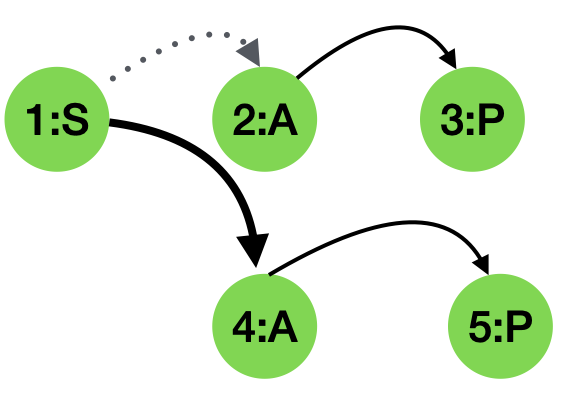
\includegraphics[width=\linewidth]{diagrams/scenarioTwo.png}
} 
\\
\hline
original configuration
&
 configuration after executing \prg{1.swap(4)}
\\
\hline \hline
\end{tabular}
   \caption{changing footprint}
   \label{fig:ScenarioA}
 \end{figure}
 
\subsection{Proving method \prg{swap}}

We can give yo  \prg{Swap}  he following pre- and post- condition pair


\subsection{First Worry}

\begin{figure}[htb]
\begin{tabular}{|c|c|cl}
\hline \\
\resizebox{4.1cm}{!}{
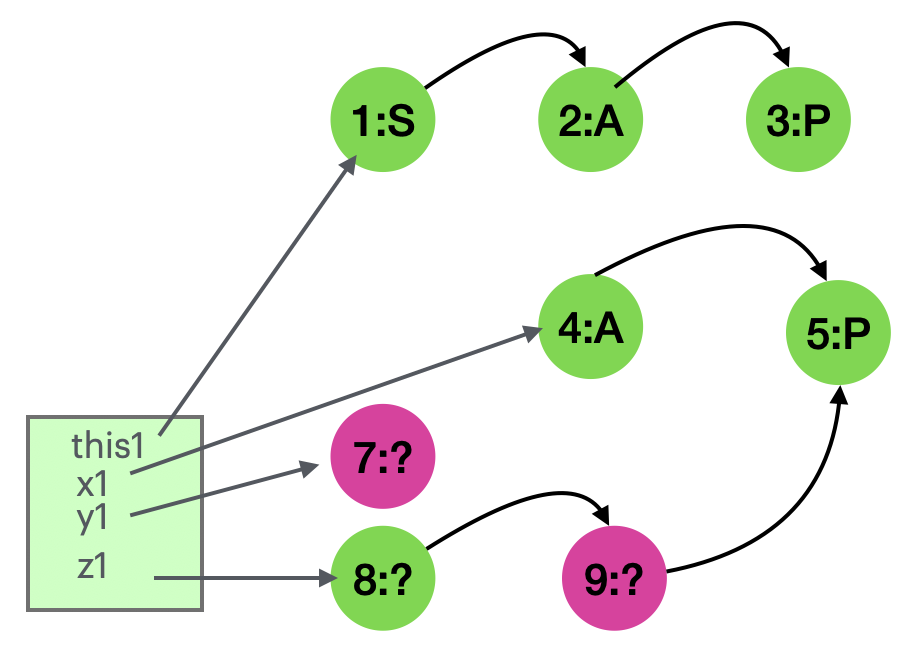
\includegraphics[width=\linewidth]{diagrams/scenarioBOne.png}
} 
&
\resizebox{4.1cm}{!}{
\includegraphics[width=\linewidth]{diagrams/scenarioBTwo.png}
} 
&
\resizebox{4.1cm}{!}{
\includegraphics[width=\linewidth]{diagrams/scenarioBThree.png}
} 
\\
\hline
$\sigma_1$
&
$\sigma_2$
&
$\sigma_3$
\\
\small{$..,\sigma_1 \models {\protectedFrom {\prg{this.acc.pwd}} {\{ \prg{x}, \prg{y}, \prg{z} \}} }$}
&
$..,\sigma_2 \models {\inside {\prg{x.acc.pwd}}}$
&
$..,\sigma_3 \models {\inside {\prg{this.acc.pwd}}} $
\\
\small{$..,\sigma_1 \not\models {\protectedFrom {\prg{x.pwd}} { \prg{z}  }}$} & & 
\\
\hline \hline
\resizebox{4.1cm}{!}{
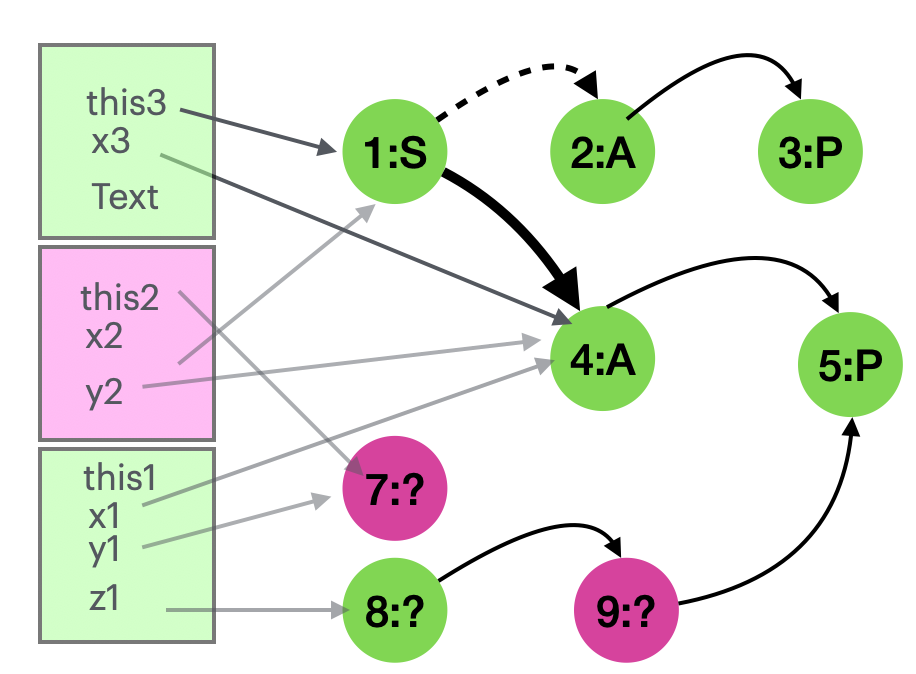
\includegraphics[width=\linewidth]{diagrams/scenarioBFour.png}
} 
&
\resizebox{4.1cm}{!}{
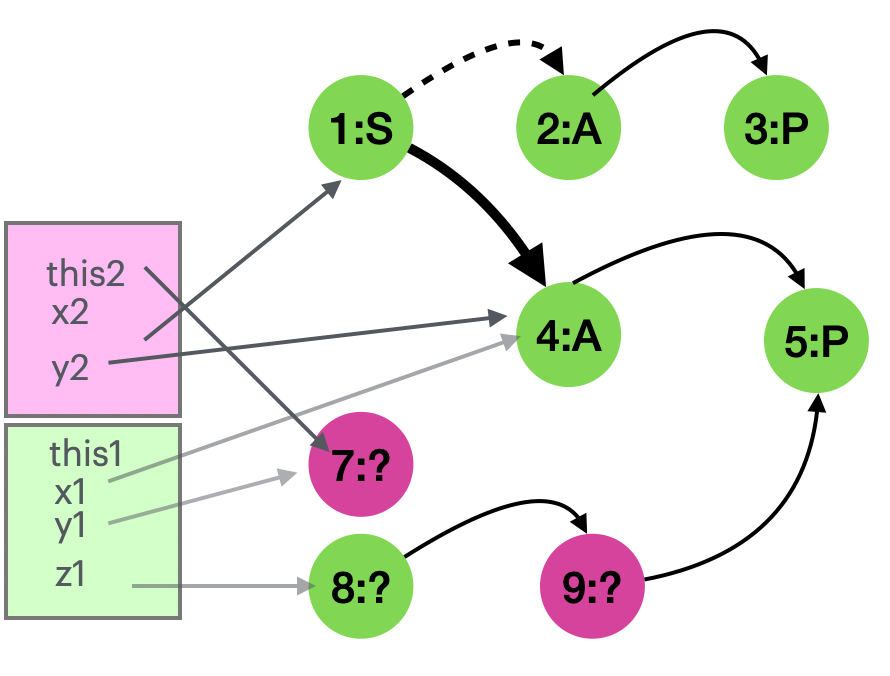
\includegraphics[width=\linewidth]{diagrams/scenarioBFive.png}
}
&
\resizebox{4.1cm}{!}{
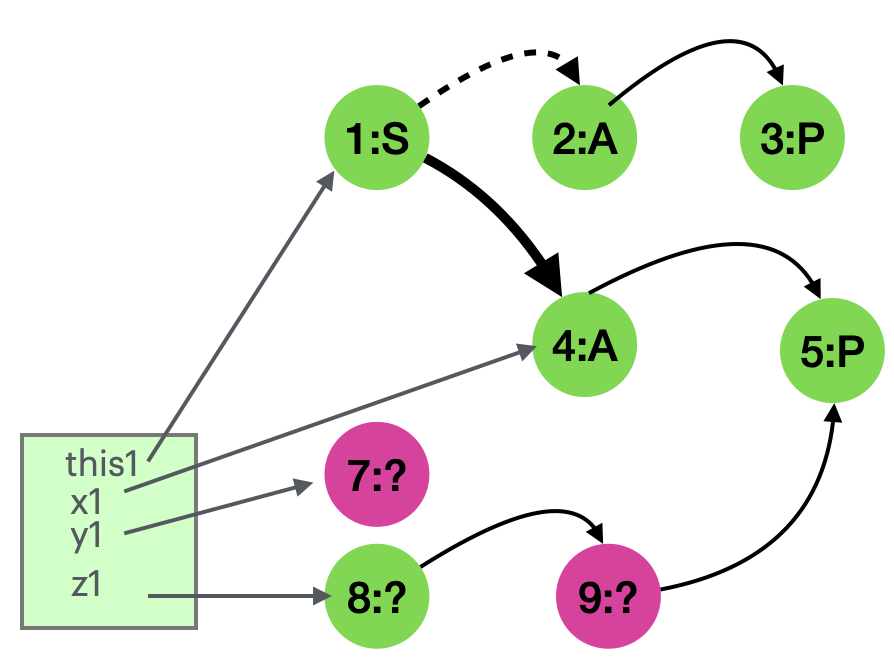
\includegraphics[width=\linewidth]{diagrams/scenarioBSix.png}
} 
\\
\hline 
$\sigma_4$
&
$\sigma_5$
&
$\sigma_6$
\\
$..,\sigma_4 \models {\inside {\prg{this.acc.pwd}}}$
&
$..,\sigma_5 \models {\inside {\prg{x.acc.pwd}}}$
&
\small{$..,\sigma_6 \not\models {\protectedFrom {\prg{this.acc.pwd}} {\{ \prg{x}, \prg{y}, \prg{z} \}} }$}
\\
\hline 
\hline
\end{tabular}
   \caption{calling \prg{swap} and exposing the password?}
   \label{fig:ScenarioB}
 \end{figure}


 
 

  
 %% Appendix
%\appendix
%\appendix
%\section{Appendix to Section \ref{sect:underlying} -- The programming language \LangOO}
\label{app:loo}


We introduce \LangOO, a simple, typed, class-based, object-oriented language.

\subsection{Syntax}

The syntax of \LangOO is given in Fig. \ref{f:loo-syntax}\footnote{{Our motivating example is provided in a slightly richer syntax for greater readability.}}.
To reduce the complexity of our formal models, as is usually done, CITE - CITE,  \LangOO lacks many
common languages features, omitting static fields and methods, interfaces,
inheritance, subsumption, exceptions, and control flow.  
 \LangOO % includes ghost fields,  that may only be used in the specification language.
and which may be defined recursively.

\LangOO modules ($M$) map class names ($C$) to class definitions ($\textit{ClassDef}$).
A class definition consists of % \jm[]{an optional annotation \enclosed},
a list of field definitions, ghost field definitions, and method definitions.
{Fields, ghost fields, and methods all have types, $C$; {types are
    classes}.
    Ghost fields may be optionally 
 annotated as \texttt{intrnl}, requiring the argument to have an internal type, and the 
body of the ghost field to only contain references to internal objects. This is enforced by the
limited type system of \LangOO.}
A program state ($\sigma$) is a pair of of a stack and a heap.
The stack is a a stack is a non-empty list of frames ($\phi$), and the heal ($\chi$)
is a map from addresses ($\alpha$) to objects ($o$). A frame consists of a local variable
map and a continuation .\prg{cont} that represents the statements that are yet to be executed ($s$).
% or a hole waiting to be filled by a method return in the frame above ($x := \bullet; s$).
A statement is either a field read ($x := y.f$), a field write ($x.f := y$), a method call
($u :=y_0.m(\overline{y})$), a constructor call ($\prg{new}\ C$), 
% a method return statement ($\prg{return}\ x$), 
  a sequence of statements ($s;\ s$),
  or empty ($\epsilon$).


\LangOO also includes syntax for expressions $\re$ that may %only
be used in writing
specifications or the definition of ghost fields.





\subsection{Semantics}
\LangOO is a simple object oriented language, and the operational semantics 
(given in Fig. \ref{f:loo-semantics} and discussed later)
do not introduce any novel or surprising features. The operational 
semantics make use of several helper definitions that we 
define here.

{
We provide a definition of reference interpretation in Definition \ref{def:interpret}
\begin{definition}
\label{def:interpret}
For a frame $\phi= (\overline {x \mapsto v}, s)$, and a program state $\sigma = (\overline \phi \cdot \phi,, \chi)$, we   define:
\begin{itemize}
\item
$\interpret{\phi}{x}\ \triangleq\ v_i$\ \ \ if \ \ \ $x=x_i$
\item
 $\interpret{\sigma}{x}\ \triangleq\  \interpret{\phi}{x}$
\item
$\interpret{\sigma}{\alpha.f}\ \triangleq\ v_i $ \ \ if \ \ $\chi(\alpha)=(\_; \  \overline {f \mapsto v})$, and $f_i=f$
\item
$\interpret{\sigma}{x.f}\ \triangleq\ \interpret{\sigma}{\alpha.f}$ where $\interpret{\sigma}{x}=\alpha$
\item
$\phi.\prg{cont} \ \triangleq\ s$ 
\item
$\sigma.\prg{cont} \ \triangleq\ \phi.\prg{cont}$\
\item
$\phi[\prg{cont}\mapsto s'] \ \triangleq\ (\overline {x \mapsto v}, s')$
\item
$\sigma[\prg{cont}\mapsto s'] \ \triangleq \ (\ {\overline \phi}\cdot \phi[\prg{cont}\mapsto s'],\  \chi\ )$ 
\item
$\phi[\prg{x'}\mapsto v'] \ \triangleq\ ( \ (\overline {x \mapsto v})[\prg{x'}\mapsto v'],\ s \ )$
\item
$\sigma[\prg{x'}\mapsto v'] \ \triangleq\ (\ (\overline {\phi} \cdot (\phi[\prg{x'}\mapsto v']), \ \chi)$ 
\item
$\sigma [\alpha \mapsto o ] \ \triangleq\ (\ (\overline {\phi} \cdot \phi), \ \chi [\alpha \mapsto o ]\ )$ 
\item
$\sigma [\alpha.f' \mapsto v' ] \ \triangleq\ \sigma [\alpha \mapsto o ] $\ \ \  if \ \  
$\chi(\alpha)=(C, {\overline {f \mapsto v}})$, and $o=(\ C;  ({\overline {f \mapsto v}})[f' \mapsto v' ]\ )$ 
\end{itemize}
\end{definition}
}
That is, a variable $x$, or a field access on a variable $x.f$ 
has an interpretation within a program state of value $v$
if $x$ maps to $v$ in the local variable map, or the field
$f$ of the object identified by $x$ points to $v$.

Definition \ref{def:class-lookup} defines the class lookup function an object 
identified by variable $x$.
\begin{definition}[Class Lookup]
\label{def:class-lookup}
For program state $\sigma = ({\overline {\phi}}\cdot\phi, \chi)$, class lookup is defined as 
$$\class{\sigma}{x}\ \triangleq\ C \ \ \ \ \ \mbox{if} \ \ \  \chi(\interpret{\sigma}{x})=(C,\_ )$$
\end{definition}

Module linking is defined for modules with disjoint definitions:

\begin{definition}
\label{def:linking}
For all modules $\Mtwo$ and $M$, if the domains of $\Mtwo$ and $M$ are disjoint, 
we define the module linking function as $M\cdot \Mtwo\ \triangleq\ M\ \cup\ M'$.
\end{definition}
That is,  their linking is the union of the two if their domains are disjoint.

Definition \ref{def:meth-lookup} defines the method lookup function for a method
call $m$ on an object of class $C$.
\begin{definition}[Method Lookup]
\label{def:meth-lookup}
For module $\Mtwo$, class $C$, and method name $m$, method lookup is defined as 
$$\meth{\Mtwo}{C}{m}\ \triangleq\ { pr}\  \prg{method}\ m\ (\overline{x : T}) {:T}\{\ s\ \}  $$
if there exists an $M$ in $\Mtwo$, so that $M(C)$ contains the definition ${ pr}\  \prg{method}\ m\ (\overline{x : T}) {:T}\{\ s\ \} $
\end{definition}

Definition \ref{def:fields-lookup} looks up all the field identifiers in a given class
\begin{definition}[Fields Lookup]
\label{def:fields-lookup}
For modules $\Mtwo$,and  class $C$, fields lookup is defined as 
$$fields(\Mtwo,C) \ \triangleq\ { pr}\ \{ \ f  \ | \  \exists  M\in\Mtwo. s.t.  M(C) \mbox{contains the definition}  \prg{field}\ f: T\ \} $$
\end{definition}



We define what it means for two objects to come from the same module
\begin{definition}[Same Module]
\label{def:same:module}
For program state $\sigma$,  modules $\Mtwo$, and variables $x$ and $y$, we defone
$$\Same {x} {y} {\sigma}{\Mtwo}\ \triangleq\ \exists C, C', M[ \ M\in \Mtwo \wedge C, C'\in M \wedge  \class{\sigma}{x}=C \wedge \class{\sigma}{y} =C'\ ]$$
\end{definition}

As we already said in \S \ref{s:underlying}, we forbid assignments to a method's parameters. 
To do that, the following function returns the  identifiers of the formal parameters of the currently active method.



\begin{definition}
For program state $\sigma$:
\label{def:params}

$\Formals \sigma \Mtwo \ \ \triangleq \ \  \overline x \ \ \ \mbox{such that} \ \  \  \exists \overline {\phi},\,\phi_k, \, \phi_{k+1}, \,C,\,p.$\\
$\strut \hspace{3.2cm} [   \ \ \sigma =  (\overline {\phi}\cdot{\phi_k}\cdot{\phi_{k+1}}\,, \chi) 
\  \ \wedge\  \ \phi_k.\prg{cont}=\_:=y_0.m(\_); \_ \  \  \wedge\ \ $\\
$\strut \hspace{3.2cm} \class{(\phi_{k+1},\chi)}  {\prg{this} }\  \ \wedge\ \ \meth{\Mtwo} {C} {m} = p \ C::m(\overline{x : \_}){:\_}\{\_\}  $
\end{definition}






% the below is now in the maintext
%Fig. \ref{f:loo-semantics} gives the operational semantics of \LangOO. 
%Program state $\sigma_1$ reduces to $\sigma_2$ in the context of
%modules$\Mtwo$ if $\exec{\Mtwo}{\sigma_1}{\sigma_2}$. The semantics in Fig. \ref{f:loo-semantics}
%are unsurprising, but it is notable that reads (\textsc{Read}) and writes (\textsc{Write})
%are restricted to the class that the field belongs to,
%{and methods  may only be called if public, or from same module as current receiver.}


\begin{figure}[hbp]
\begin{minipage}{\textwidth}
\footnotesize{
\begin{mathpar}
\infer
		{}
		{\eval{M}{\sigma}{v}{v}}
		\quad(\textsc{E-Val})
		\and
\infer
		{}
		{\eval{M}{\sigma}{x}{\interpret{\sigma}{x}}}
		\quad(\textsc{E-Var})
		\and
%\infer
%		{
%		\eval{M}{\sigma}{e_1}{i_1}\\
%		\eval{M}{\sigma}{e_2}{i_2}\\
%		i_1 + i_2 = i
%		}
%		{
%		\eval{M}{\sigma}{e_1 + e_2}{i}
%		}
%		\quad(\textsc{E-Add})
%		\and
%\infer
%		{
%		\eval{M}{\sigma}{e_1}{v}\\
%		\eval{M}{\sigma}{e_2}{v}
%		}
%		{
%		\eval{M}{\sigma}{e_1 = e_2}{\true}
%		}
%		\quad(\textsc{E-Eq}_1)
%		\and
%\infer
%		{
%		\eval{M}{\sigma}{e_1}{v_1}\\
%		\eval{M}{\sigma}{e_2}{v_2}\\
%		v_1 \neq\ v_2
%		}
%		{
%		\eval{M}{\sigma}{e_1 = e_2}{\false}
%		}
%		\quad(\textsc{E-Eq}_2)
%		\and
%\infer
%		{
%		\eval{M}{\sigma}{e}{\true}\\
%		\eval{M}{\sigma}{e_1}{v}
%		}
%		{
%%		\eval{M}{\sigma}{\ifthenelse{e}{e_1}{e_2}}{v}
%		\eval{M}{\sigma}{e}{v}
%		}
%		\quad(\textsc{E-If}_1)
%		\and
%\infer
%		{
%		\eval{M}{\sigma}{e}{\false}\\
%		\eval{M}{\sigma}{e_2}{v}
%		}
%		{
%%		\eval{M}{\sigma}{\ifthenelse{e}{e_1}{e_2}}{v}
%		\eval{M}{\sigma}{e}{v}
%		}
%		\quad(\textsc{E-If}_2)
%		\and
\infer
		{
		\eval{M}{\sigma}{\re}{\alpha}
		}
		{
		\eval{M}{\sigma}{\re.f}{\interpret{\sigma}{\alpha.f}}
		}
		\quad(\textsc{E-Field})
		\and
\infer
		{
		\eval{M}{\sigma}{\re_0}{\alpha}\\
		\overline {\eval{M}{\sigma}{\re}{v}}\\
		M(\class{\sigma}{\alpha})\ \mbox{contains}\ \prg{ghost}\ gf(\overline{x : T)}\{\re\} : T' \\
		\eval{M}{\sigma}{[\overline {v/x}]\re}{v}
		}
		{
		\eval{M}{\sigma}{\re_0.gf(\overline{\re})}{v}
		}
		\quad(\textsc{E-Ghost})
\end{mathpar}
}
\caption{\LangOO Expression evaluation}
\label{f:evaluation}
\end{minipage}
\end{figure}

While the small-step operational semantics of \LangOO is given in Fig. \ref{f:loo-semantics},
specification satisfaction is defined over an abstracted notion of 
the operational semantics that models the open world. %, called \jm[]{\emph{external states semantics}}. 




An \emph{Initial} program state contains a single frame 
with a single local variable \prg{this} pointing to a single object 
in the heap of class \prg{Object}, and a continuation.
\begin{definition}[Initial Program State]
\label{def:initial}
A program state $\sigma$ is said to be an initial state ($\initial{\sigma}$)
if and only if
\begin{itemize}
\item
$\sigma\ =\  ( ((\prg{this}\ \mapsto\ \alpha), s); \  (\alpha \mapsto (\prg{Object}, \emptyset)$
\end{itemize} 
for some address $\alpha$ and some statement $s$.
\end{definition}


%We give the semantics of module pair execution in Definition \ref{def:pair-reduce}
%\begin{definition}[External State Semantics]
%\label{def:pair-reduce-appendix}
%For all internal modules $M_1$, external modules $M_2$, and program configurations $\sigma$ and $\sigma'$, 
%we say that $\reduction{M_1}{M_2}{\sigma}{\sigma'}$ if and only if
%\begin{itemize}
%\item
%$\class{\sigma}{\sigma(\prg{this})}\ \in\ M_2$ and
%\item
%$\class{\sigma'}{\sigma'(\prg{this})}\ \in\ M_2$ and 
%\end{itemize} 
%and
%\begin{itemize}
%\item
%$\exec{M_1\ \circ\ M_2}{\sigma}{\sigma'}$ or
%\item
%$M_1 \circ M_2, \sigma \leadsto \sigma_1 \leadsto \ldots \sigma_n \leadsto \sigma'$ and $\class{\sigma_i}{\sigma_i(\prg{this})} \in M_1$ for all $1 \leq i \leq\ n$
%\end{itemize}
%\end{definition}

We provide a semantics for expression evaluation is given in Fig. \ref{f:evaluation}. 
That is, given a module $M$ and a program state $\sigma$, expression $e$ evaluates to $v$
if $\eval{M}{\sigma}{e}{v}$. Note, the evaluation of expressions is separate from the operational
semantics of \LangOO, and thus there is no restriction on field access.

{
\paragraph{Lemmas and Proofs}
}
%We prove lemma  \ref{l:var:unaffect}, using the following lemma:

%\begin{lemma}
%\label{l:leadsto:depth}
%For any states $\sigma$, $\sigma'$, modules $\Mtwo$,  number $k$, and variable $y$:
%
%\begin{enumerate}
%\item
%$ \EarlierS {\sigma}  {\sigma'}\ \ \Longrightarrow \ \ \DepthSt {\sigma} \leq \DepthSt {\sigma}$.
%
%\item
%$\leadstoBoundedThree   {\Mtwo}  {\sigma_1} {\sigma}  {\sigma_2}\ \  \ \Longrightarrow\ \ \ \DepthSt {\sigma} \leq \DepthSt {\sigma_1}\ \wedge \ \DepthSt {\sigma} \leq \DepthSt {\sigma_2}$.
%
%\item
%$\leadstoBoundedThree   {\Mtwo}  {\sigma_1} {\sigma}  {\sigma_2}\ \wedge\ 
% k=    \DepthSt \sigma \ \wedge\ (k <\DepthSt {\sigma_1} \vee k < \DepthSt {\sigma_2})\ \ \ \Longrightarrow \ \ \
%\interpret {\sigma} {y} = \interpret {\RestictTo {\sigma_1} {k}} y= \interpret {\RestictTo {\sigma_2} {k}} y .$
%
%\item
%$\leadstoOrig {\Mtwo} {\sigma} {\sigma'}\ \  \wedge\  \  \DepthSt \sigma = \DepthSt {\sigma'} \ \ \wedge \ \
%y\notin \vs(\sigma.\prg{cont}) \ \ \Longrightarrow \ \  \interpret \sigma y =  \interpret {\sigma'} y$
% 
%\end{enumerate}
%\end{lemma}
%}
% 
%{
%\beginProof{l:leadsto:depth}
%\begin{enumerate}
%\item Follows from the definition of $\DepthSt {\_}$, and $ \EarlierS {\_}  {\_}$.
%\item Follows from the definition  $\leadstoBoundedThree {\_} {\_} {\_} {\_}$ and (1).
% 
%\item  From. $\leadstoBoundedThree   {\Mtwo}  {\sigma_1} {\sigma}  {\sigma_2}\ \wedge\ 
% k= \DepthSt \sigma \ \wedge\ (k <\DepthSt {\sigma_1} \vee k < \DepthSt {\sigma_2})$ we can deduce that the step from $\sigma_1$ to $\sigma_2$ 
% is either a method call from $\sigma$, 
% ????
% 
%\item
%Follows from the operational semantics
%
%\end{enumerate}
%\completeProof
%}

 
\beginProof{l:wf:state}
\sdred{The first assertion is proven by unfolding the definition of $\_ \models \_ $.

The second assertion is proven by case analysis on the execution relation $\exec {\_} {\sigma} {\sigma'}$. 
The assertion gets established when we call a method, and is preserved through all the execution steps, because we do not allow assignments to the formal parameters.
 
}
\completeProof

We now prove lemma \ref{l:var:unaffect}:

\beginProof{l:var:unaffect} 
\begin{itemize}
\item
We first show that $\leadstoBoundedThree {\Mtwo} {\sigma} {\sigma\bd}  {\sigma'}   \ \wedge \ k<\DepthSt \sigma\bd  \ \ \Longrightarrow \ \  \interpret {\RestrictTo \sigma k} y =  \interpret {\RestrictTo {\sigma'} k} y$
This follows easily from the operational semantics, and the definitions.


\item
By induction on the earlier part, we  obtain that $\leadstoBoundedStar {\Mtwo}  {\sigma}  {\sigma'}  \ \wedge \ k<\DepthSt \sigma  \ \ \Longrightarrow \ \  \interpret {\RestrictTo \sigma k} y =  \interpret {\RestrictTo {\sigma'} k} y$

\item

We now show that $\leadstoBoundedStarFin {\Mtwo}  {\sigma}  {\sigma'} \ \wedge \ y\notin \vs(\sigma.\prg{cont}) \ \ \Longrightarrow \ \  \interpret \sigma y =  \interpret {\sigma'} y$ by  induction on the number of steps, and  using the earlier lemma.
\end{itemize}
\completeProof

\sdred{Lemma \ref{lemma:relevant:more} states that initila states are well-formed, and that (\ref{threeLR}) a pre-existing object, locally reachable after any number of scoped execution steps, was locally reachable at the first step.


\begin{lemma}
\label{lemma:relevant:more}
For all modules $\Mtwo$, states $\sigma$, $\sigma'$,   and frame $\phi$:
\begin{enumerate}
\item
\label{lemma:relevant:more:one}
$\initial {\sigma}  \ \    \Longrightarrow \ \ \Mtwo \models \sigma $
\item
\label{threeLR}
{${\leadstoBoundedStar {\Mtwo}  {\sigma}    {\sigma'}}  \ \  \Longrightarrow\ \ 
dom(\sigma) \cap \LRelevantO {\sigma'} \subseteq   \LRelevantO {\sigma}$
}

\end{enumerate}
\end{lemma}

{Consider Fig.  \ref{fig:illusrPreserve} . %, and Fig.  \ref{fig:UpSemanticsBounded}.
Lemma \ref{lemma:relevant:more}, part \ref{threeLR}  promises that any objects locally reachable in $\sigma_{14}$ which already existed in $\sigma_{8}$, were locally reachable in $\sigma_{8}$. However, the lemma is only  applicable to scoped execution, and as 
$\notLeadstoBoundedStar {\Mtwo} {\sigma_8}  {\sigma_{17}}$, 
the lemma does not promise that  objects locally reachable in $\sigma_{17}$ which already existed in $\sigma_{8}$, were locally accessible in $\sigma_{8}$ -- namely it could be that objects are made globally reachable upon method return, during the step from $\sigma_{14}$ to $\sigma_{15}$.}
}




%\clearpage
%\section{Encapsulation}
%

\subsection{Proving Encapsulation}
\label{s:encap-proof}

%We start by giving providing the syntax for type contexts in Fig. \ref{f:context-syntax}.
%\begin{figure}[t]
%\[
%\begin{syntax}
%\syntaxElement{\Gamma}{Type Context}
%		{
%		\syntaxline
%				{\emptyset}
%				{\alpha : C,\ \Gamma}
%		\endsyntaxline
%		}
%\endSyntaxElement\\
%\end{syntax}
%\]
%\caption{}
%\label{f:context-syntax}
%\end{figure}
%We construct type contexts out of assertions using the following rules:
%\begin{mathpar}
%\infer
%		{}
%		{\textit{Env}(\alpha : C) = \alpha : C,\ \emptyset}
%		\and
%\infer
%		{}
%		{\textit{Env}(A_1\ \wedge\ A_2) = \textit{Env}(A_1) \cup \textit{Env}(A_2)}
%\end{mathpar}
%\begin{definition}[Assertion Encapsulation]
%For all modules $M$, and assertions $A$, and $A'$ we say $M\ \vdash\ A\ \Rightarrow\ A'$ if and only if M
%\end{definition}
We provide a simple inference system for assertion encapsulation (Definition \ref{def:encapsulation}),
that is proving a change in satisfaction of an assertion depends on computation from the internal module. 
As encapsulation is not the core topic of this paper, we keep this relatively simple. As discussed before, 
we assume the existence of a simple ownership type system to ensure certain forms of encapsulation.

To assist in the definition of a proof system to proof assertion encapsulation,
we define proof rules for expressions that depend entirely on internal objects (or primitves)
for their evaluation.
\begin{definition}[Internal Expressions]
For all modules $M$, assertions $A$, and expressions $e$, 
$\satisfies{M}{\givenA{A}{\intrnl{e}}}$ if and only if for all external modules 
$M'$, heaps $\chi$, frame stacks $\psi$, and values $v$,
such that $\satisfiesA{M}{M'}{(\chi, \psi)}{A}$ and
$\eval{M \circ M'}{(\chi, \psi)}{e}{v}$
then 
$\eval{M \circ M'}{(\chi', \psi)}{e}{v}$, 
where $\chi'$ is the portion of $\chi$ internal to $M$, i.e. 
$\chi' = \{[\alpha \mapsto o]| [\alpha \mapsto o] \in \chi\ \textit{and}\ o.(\prg{class}) \in M \}$
\end{definition}


The encapsulation proof system thus consists of two relations 
\begin{itemize}
\item
Purely internal expressions: $\proves{M}{\givenA{A}{\intrnl{e}}}$ and
\item
Assertion encapsulation: $\proves{M}{\givenA{A}{\encaps{A'}}}$
\end{itemize}

Fig. \ref{f:intrnl} gives proof rules for evaluation of an expression comprising of purely module internal objects.
Fig. \ref{f:asrt-encap} gives proof rules for whether an assertion is encapsulated, that is whether 
a change in satisfaction of an assertion requires interaction with the internal module.

\begin{figure}[t]
\footnotesize
\begin{mathpar}
\infer
		{}
		{\proves{M}{\givenA{A}{\intrnl{i}}}}
		\quad(\textsc{Intrnl-Int})
		\and
\infer
		{}
		{\proves{M}{\givenA{A}{\intrnl{\nul}}}}
		\and
\infer
		{}
		{\proves{M}{\givenA{A}{\intrnl{\true}}}}
		\and
\infer
		{}
		{\proves{M}{\givenA{A}{\intrnl{\false}}}}
		\and
\infer
		{
		\proves{M}{A\ \longrightarrow\ \alpha : C}\\
		C\ \in\ M
		}
		{
		\proves{M}{\givenA{A}{\intrnl{\alpha}}}
		}
		\quad(\textsc{Intrnl-Obj})
		\and
\infer
		{
		\proves{M}{\givenA{A}{\intrnl{e}}}\\
		\proves{M}{A\ \longrightarrow\ e : C}\\
		[\prg{field}\ \_\ f\ :\ D]\ \in\ M(C).(\prg{flds}) \\
		D\ \in\ M
		}
		{
		\proves{M}{\givenA{A}{\intrnl{e.f}}}
		}
		\quad(\textsc{Intrnl-Field})
		\and
\infer
		{
		\proves{M}{\givenA{A}{\intrnl{e_1}}}\\
		\proves{M}{\givenA{A}{\intrnl{e_2}}}\\
%		\proves{M}{\givenA{A}{\intrnl{e}}} \\
		\proves{M}{A\ \longrightarrow\ e_1 : C} \\
		\prg{ghost}\ \prg{intrnl}\ g(x : \_)\{e\} \in M(C).(\prg{gflds})
		}
		{
		\proves{M}{\givenA{A}{\intrnl{e_1.g(e_2)}}}
		}
		\quad(\textsc{Intrnl-Ghost})
\end{mathpar}
\caption{Internal Proof Rules}
\label{f:intrnl}
\end{figure}

\begin{figure}[t]
\footnotesize
\begin{mathpar}
\infer
		{\proves{M}{\givenA{A}{\intrnl{e}}}}
		{\proves{M}{\givenA{A}{\encaps{e}}}}
		\quad(\textsc{Enc-Intrnl})
		\and
\infer
		{\proves{M}{\givenA{A}{\intrnl{e}}}}
		{\proves{M}{\givenA{A}{\encaps{e.f}}}}
		\and
\infer
		{
		\proves{M}{\givenA{A}{\encaps{e_1}}} \\
		\proves{M}{\givenA{A}{\encaps{e_2}}}
		}
		{
		\proves{M}{\givenA{A}{\encaps{e_1 = e_2}}}
		}
		\and
\infer
		{
		\proves{M}{\givenA{A}{\encaps{e_1}}} \\
		\proves{M}{\givenA{A}{\encaps{e_2}}}
		}
		{
		\proves{M}{\givenA{A}{\encaps{e_1 + e_2}}}
		}
		\and
\infer
		{
		\proves{M}{\givenA{A}{\encaps{e_1}}} \\
		\proves{M}{\givenA{A}{\encaps{e_2}}}
		}
		{
		\proves{M}{\givenA{A}{\encaps{e_1 < e_2}}}
		}
		\and
\infer
		{
		\proves{M}{\givenA{A}{\encaps{e}}} \\
		\proves{M}{\givenA{A}{\encaps{e_1}}} \\
		\proves{M}{\givenA{A}{\encaps{e_2}}}
		}
		{
		\proves{M}{\givenA{A}{\encaps{\prg{if}\ e\ \prg{then}\ e_1\ \prg{else}\ e_2}}}
		}
		\and
\infer
		{\proves{M}{A\ \longrightarrow\ \internal{\alpha_1}}}
		{\proves{M}{\givenA{A}{\encaps{\access{\alpha_1}{\alpha_2}}}}}
		\and
\infer
		{}
		{\proves{M}{\givenA{A}{\encaps{\wrapped{\alpha}}}}}
		\quad(\textsc{Enc-Wrapped})
		\and
\infer
		{\proves{M}{A\ \longrightarrow\ \wrapped{\alpha_2}}}
		{\proves{M}{\givenA{A}{\encaps{\neg \access{\alpha_1}{\alpha_2}}}}}
		\and
\infer
		{
		\proves{M}{A_1\ \longrightarrow\ A_2} \\
		\proves{M}{A\ \longrightarrow\ A_1} \\
		\proves{M}{\givenA{A}{\encaps{A_1}}}
		}
		{\proves{M}{\givenA{A}{\encaps{A_2}}}}
\end{mathpar}
\caption{Assertion Encapsulation Proof Rules}
\label{f:asrt-encap}
\end{figure}
%\clearpage
%\section{More about the Expressiveness of \Nec Specifications}
\label{s:expressiveness:appendix}

 %% We continue the comparison of expresiveness between \emph{Chainmail} and \Nec, by 
 %% considering the examples studied in \cite{FASE}.
 
\subsection{ERC20}
The ERC20 \cite{ERC20} is a widely used token standard describing the basic functionality of any Ethereum-based token 
contract. This functionality includes issuing tokens, keeping track of tokens belonging to participants, and the 
transfer of tokens between participants. Tokens may only be transferred if there are sufficient tokens in the 
participant's account, and if either they (using the \prg{transfer} method) or someone authorized by the participant (using the \prg{transferFrom} method) initiated the transfer. 

We specify these necessary conditions here using \Nec. Firstly, \prg{ERC20Spec1} 
says that if the balance of a participant's account is ever reduced by some amount $m$, then
that must have occurred as a result of a call to the \prg{transfer} method with amount $m$ by the participant,
or the \prg{transferFrom} method with the amount $m$ by some other participant.
\begin{lstlisting}[language = Chainmail, mathescape=true, frame=lines]
ERC20Spec1 $\triangleq$ from e : ERC20 $\wedge$ e.balance(p) = m + m' $\wedge$ m > 0
              next e.balance(p) = m'
              onlyIf $\exists$ p' p''.[$\calls{\prg{p'}}{\prg{e}}{\prg{transfer}}{\prg{p, m}}$ $\vee$ 
                     e.allowed(p, p'') $\geq$ m $\wedge$ $\calls{\prg{p''}}{\prg{e}}{\prg{transferFrom}}{\prg{p', m}}$]
\end{lstlisting}
Secondly, \prg{ERC20Spec2} specifies under what circumstances some participant \prg{p'} is authorized to 
spend \prg{m} tokens on behalf of \prg{p}: either \prg{p} approved \prg{p'}, \prg{p'} was previously authorized,
or \prg{p'} was authorized for some amount \prg{m + m'}, and spent \prg{m'}.
\begin{lstlisting}[language = Chainmail, mathescape=true, frame=lines]
ERC20Spec2 $\triangleq$ from e : ERC20 $\wedge$ p : Object $\wedge$ p' : Object $\wedge$ m : Nat
              next e.allowed(p, p') = m
              onlyIf $\calls{\prg{p}}{\prg{e}}{\prg{approve}}{\prg{p', m}}$ $\vee$ 
                     (e.allowed(p, p') = m $\wedge$ 
                      $\neg$ ($\calls{\prg{p'}}{\prg{e}}{\prg{transferFrom}}{\prg{p, \_}}$ $\vee$ 
                              $\calls{\prg{p}}{\prg{e}}{\prg{allowed}}{\prg{p, \_}}$)) $\vee$
                     $\exists$ p''. [e.allowed(p, p') = m + m' $\wedge$ $\calls{\prg{p'}}{\prg{e}}{\prg{transferFrom}}{\prg{p'', m'}}$]
\end{lstlisting}

\subsection{DAO}
The Decentralized Autonomous Organization (DAO)~\cite{Dao}  is a well-known Ethereum contract allowing 
participants to invest funds. The DAO famously was exploited with a re-entrancy bug in 2016, 
and lost \$50M. Here we provide specifications that would have secured the DAO against such a 
bug. \prg{DAOSpec1} says that no participant's balance may ever exceed the ether remaining 
in DAO.
\begin{lstlisting}[language = Chainmail, mathescape=true, frame=lines]
DAOSpec1 $\triangleq$ from d : DAO $\wedge$ p : Object
            to d.balance(p) > d.ether
            onlyIf false
\end{lstlisting}
Note that \prg{DAOSpec1} enforces a class invariant of \prg{DAO}, something that could be enforced
by traditional specifications using class invariants.
The second specification \prg{DAOSpec2} states that if after some single step of execution, a participant's balance is \prg{m}, then 
either 
\begin{description}
\item[(a)] this occurred as a result of joining the DAO with an initial investment of \prg{m}, 
\item[(b)] the balance is \prg{0} and they've just withdrawn their funds, or 
\item[(c) ]the balance was \prg{m} to begin with
\end{description}
\begin{lstlisting}[language = Chainmail, mathescape=true, frame=lines]
DAOSpec2 $\triangleq$ from d : DAO $\wedge$ p : Object
            next d.balance(p) = m
            onlyIf $\calls{\prg{p}}{\prg{d}}{\prg{repay}}{\prg{\_}}$ $\wedge$ m = 0 $\vee$ $\calls{\prg{p}}{\prg{d}}{\prg{join}}{\prg{m}}$ $\vee$ d.balance(p) = m
\end{lstlisting}

\sophiaPonder[small changes over Julian's]{\subsection{Safe}
\cite{FASE} used as a running example   a Safe, where a treasure 
was secured within a \texttt{Safe} object, and access to the treasure was only granted by 
providing the correct password. }
\ Using \Nec, we express \texttt{SafeSpec}, that requires that the treasure cannot be 
removed from the safe without knowledge of the secret.
\begin{lstlisting}[language = Chainmail, mathescape=true, frame=lines]
SafeSpec $\triangleq$ from s : Safe $\wedge$ s.treasure != null
            to s.treasure == null
            onlyIf $\neg$ inside(s.secret)
\end{lstlisting}

The module  \prg{SafeModule} described  below satisfies  \prg{SafeSpec}.

\begin{lstlisting}[frame=lines]
module SafeModule
     class Secret{}
     class Treasure{}
     class Safe{
         field treasure : Treasure
         field secret : Secret
         method take(scr : Secret){
              if (this.secret==scr) then {
                   t=treasure
                   this.treasure = null
                   return t } 
          }
 }
\end{lstlisting}

 

%\clearpage
%\section{More \Nec Logic rules}
%\label{a:necSpec}
%
\begin{figure}[t]
\footnotesize
\begin{mathpar}
\infer
	{\proves{M}{\onlyIfSingle{A}{\neg A}{A'}}}
	{
	\proves{M}{\onlyThrough{A}{\neg A}{A'}}
	}
	\quad(\textsc{Changes})
	\and
\infer
	{
	\proves{M}{A_1\ \longrightarrow\ A_1'}\\
	\proves{M}{A_2\ \longrightarrow\ A_2'}\\
	\proves{M}{A_3'\ \longrightarrow\ A_3}\\
	\proves{M}{\onlyThrough{A_1'}{A_2'}{A_3'}}
	}
	{\proves{M}{\onlyThrough{A_1}{A_2}{A_3}}}
	\quad(\textsc{$\longrightarrow$})
	\and
\infer
	{
	\proves{M}{\onlyThrough{A_1}{A_2}{A}} \\\\
	\proves{M}{\onlyThrough{A_1'}{A_2}{A'}}
	}
	{\proves{M}{\onlyThrough{A_1\ \vee\ A_1'}{A_2}{A\ \vee\ A'}}}
	\quad(\textsc{$\vee$I$_1$})
	\and
\infer
	{
	\proves{M}{\onlyThrough{A_1}{A_2}{A}} \\\\
	\proves{M}{\onlyThrough{A_1}{A_2'}{A'}}
	}
	{\proves{M}{\onlyThrough{A_1}{A_2\ \vee\ A_2'}{A\ \vee\ A'}}}
	\quad(\textsc{$\vee$I$_2$})
	\and
\infer
	{
	\proves{M}{\onlyThrough{A_1}{A'}{\prg{false}}} \\\\
	\proves{M}{\onlyThrough{A_1}{A_2}{A\ \vee\ A'}}
	}
	{\proves{M}{\onlyThrough{A_1}{A_2}{A}}}
	\quad(\textsc{$\vee$E$_1$})
	\and
\infer
	{
	\proves{M}{\onlyThrough{A'}{A_2}{\prg{false}}} \\\\
	\proves{M}{\onlyThrough{A_1}{A_2}{A\ \vee\ A'}}
	}
	{\proves{M}{\onlyThrough{A_1}{A_2}{A}}}
	\quad(\textsc{$\vee$E$_2$})
	\and
\infer
	{
	\proves{M}{\onlyThrough{A_1}{A_2}{A_3}} \\\\
	\proves{M}{\onlyThrough{A_1}{A_3}{A}}
	}
	{\proves{M}{\onlyThrough{A_1}{A_2}{A}}}
	\quad(\textsc{Trans$_1$})
	\and
\infer
	{
	\proves{M}{\onlyThrough{A_1}{A_2}{A_3}} \\\\
	\proves{M}{\onlyThrough{A_3}{A_2}{A}}
	}
	{\proves{M}{\onlyThrough{A_1}{A_2}{A}}}
	\quad(\textsc{Trans$_2$})
	\and
\infer
	{
	\proves{M}{\onlyIf{A_1}{A_2}{A}}
	}
	{\proves{M}{\onlyThrough{A_1}{A_2}{A}}}
	\quad(\textsc{If})
	\and
\infer
	{}
	{\proves{M}{\onlyThrough{A_1}{A_2}{A_2}}}
	\quad(\textsc{End})
	\and
\infer
	{
	\forall y,\; \proves{M}{\onlyThrough{([y / x]A_1)}{A_2}{A}}
	}
	{\proves{M}{\onlyThrough{\exists x. [A_1]}{A_2}{A}}}
	\quad(\textsc{$\exists_1$})
	\and
\infer
	{
	\forall y,\; \proves{M}{\onlyThrough{A_1}{([y / x]A_2)}{A}}
	}
	{\proves{M}{\onlyThrough{A_1}{A_2}{A}}}
	\quad(\textsc{$\exists_2$})
\end{mathpar}
\caption{\emph{Only Through}}
\label{app:f:only-through}
\end{figure}
\begin{figure}[t]
\footnotesize
\begin{mathpar}
\infer
	{
	\proves{M}{A_1\ \longrightarrow\ A_1'}\\
	\proves{M}{A_2\ \longrightarrow\ A_2'}\\
	\proves{M}{A_3'\ \longrightarrow\ A_3}\\
	\proves{M}{\onlyIf{A_1'}{A_2'}{A_3'}}
	}
	{\proves{M}{\onlyIf{A_1}{A_2}{A_3}}}
	\quad(\textsc{If-$\longrightarrow$})
	\and
\infer
	{
	\proves{M}{\onlyIf{A_1}{A_2}{A}} \\\\
	\proves{M}{\onlyIf{A_1'}{A_2}{A'}}
	}
	{\proves{M}{\onlyIf{A_1\ \vee\ A_1'}{A_2}{A\ \vee\ A'}}}
	\quad(\textsc{If-$\vee$I$_1$})
	\and
\infer
	{
	\proves{M}{\onlyIf{A_1}{A_2}{A}} \\\\
	\proves{M}{\onlyIf{A_1}{A_2'}{A'}}
	}
	{\proves{M}{\onlyIf{A_1}{A_2\ \vee\ A_2'}{A\ \vee\ A'}}}
	\quad(\textsc{If-$\vee$I$_2$})
	\and
\infer
	{
	\proves{M}{\onlyIf{A_1}{A_2}{A\ \vee\ A'}} \\\\
	\proves{M}{\onlyThrough{A'}{A_2}{\prg{false}}}
	}
	{\proves{M}{\onlyIf{A_1}{A_2}{A}}}
	\quad(\textsc{If-$\vee$E})
	\and
\infer
	{
	\proves{M}{\onlyIf{A_1}{A_2}{A}} \\\\
	\proves{M}{\onlyThrough{A_1}{A_2}{A'}}
	}
	{\proves{M}{\onlyIf{A_1}{A_2}{A\ \wedge\ A'}}}
	\quad(\textsc{If-$\wedge$I})
	\and
\infer
	{
	\proves{M}{\onlyThrough{A_1}{A_2}{A_3}} \\\\
	\proves{M}{\onlyIf{A_1}{A_3}{A}}
	}
	{\proves{M}{\onlyIf{A_1}{A_2}{A}}}
	\quad(\textsc{If-Trans)}
	\and
\infer
	{}
	{\proves{M}{\onlyIf{A_1}{A_2}{A_1}}}
	\quad(\textsc{If-Start})
	\and
\infer
	{
	\forall y,\; \proves{M}{\onlyIf{([y / x]A_1)}{A_2}{A}}
	}
	{\proves{M}{\onlyIf{\exists x. [A_1]}{A_2}{A}}}
	\quad(\textsc{If-$\exists_1$})
	\and
\infer
	{
	\forall y,\; \proves{M}{\onlyIf{A_1}{([y / x]A_2)}{A}}
	}
	{\proves{M}{\onlyIf{A_1}{A_2}{A}}}
	\quad(\textsc{If-$\exists_2$})
\end{mathpar}
\caption{\emph{Only If}}
\label{app:f:only-if}
\end{figure}
%\clearpage
%\newpage
\section{\SpecO Logic}
\label{app:assert_logic}


{
\begin{figure}[ht]
\footnotesize
\begin{mathpar}
\infer
		{}
		{\proves{M}{\calls{x}{y}{m}{\overline{z}}\ \longrightarrow\ \external{x}}}
		\quad(\textsc{Caller-Ext})
		\and
\infer
		{}
		{\proves{M}{\calls{x}{y}{m}{\overline{z}}\ \longrightarrow\ \access{x}{y}}}
		\quad(\textsc{Caller-Recv})
		\and
\infer
		{}
		{\proves{M}{\calls{x}{y}{m}{\ldots, z_i, \ldots}\ \longrightarrow\ \access{x}{z_i}}}
		\quad(\textsc{Caller-Args})
		\and
\infer
		{C \in M}
		{\proves{M}{x\ :\ C\ \longrightarrow\ \internal{x}}}
		\quad(\textsc{Class-Int})
		\and
\infer
		{(\prg{field}\ \_\ f\ :\ D)\ \in\ M(C).(\prg{flds})}
		{\proves{M}{e : C\ \longrightarrow\ e.f : D}}
		\quad(\textsc{Fld-Class})
		\and
\infer
		{(\prg{class}\ \enclosed\ C \{\_; \_\})\ \in\ M}
		{\proves{M}{x : C\ \longrightarrow\ \wrapped{x}}}
		\quad(\textsc{Inside-Int})
		\and
\infer
		{}
		{\proves{M}{\false\ \longrightarrow\ A}}
		\quad(\textsc{Absurd})
		\and
\infer
		{}
		{\proves{M}{A\ \vee\ \neg A}}
		\quad(\textsc{Excluded Middle})
\end{mathpar}
\normalsize
\caption{Assumed Properties of the \SpecO proof system.}
\label{f:assertProperties}
\end{figure}}

In Fig. \ref{f:assertProperties} we present some assumed rules of the 
\SpecO proof system, of the form $\proves{M}{A}$. These rules
are relatively simple, with none assuming any surprising results.
They are straightforward, and would be easy to prove sound. 
\textsc{Caller-Ext}, \textsc{Caller-Recv}, \textsc{Caller-Args},
and \textsc{Class-Int} are simple properties that arise from 
the semantics of \SpecO.
\textsc{Fld-Class} and \textsc{Inside-Int} are directly drawn from 
the simple type system of \Loo.
\textsc{Absurd} and \textsc{Excluded Middle} are common logical properties.
%\clearpage
%\newpage
\section{Bank Account Example}
\label{app:BankAccount}


\begin{figure}[ht]
\begin{lstlisting}[mathescape=true, frame=lines]
module $\ModD$
  class Account
    field password : Object
    method authenticate(pwd : Object) : bool
      (PRE:  a : Account $\wedge$ b : Bank
       POST: b.balance(a)$_\prg{old}$ == b.balance(a)$_\prg{new}$)
      (PRE:  a : Account
       POST: res != a.password)
      (PRE:  a : Account
       POST: a.password$_\prg{old}$ == a.password$_\prg{new}$)
      {return pwd == this.password}
    method changePassword(pwd : Object, newPwd : Object) : void
      (PRE:  a : Account
       POST: res != a.password)
      (PRE:  a : Account $\wedge$ b : Bank
       POST: b.balance(a)$_\prg{old}$ == b.balance(a)$_\prg{new}$)
      (PRE:  a : Account $\wedge$ pwd != this.password
       POST: a.password$_\prg{old}$ = a.password$_\prg{new}$)
      {if pwd == this.password
        this.password := newPwd}

  class confined Ledger
    field acc1 : Account
    field bal1 : int
    field acc2 : Account
    field bal2 : int
    ghost intrnl balance(acc) : int = 
      if acc == acc1
        bal1
      else if acc == acc2
        bal2
      else -1
    method transfer(amt : int, from : Account, to : Account) : void
      (PRE:  a : Account $\wedge$ b : Bank $\wedge$ (a != acc1 $\wedge$ a != acc2)
       POST: b.balance(a)$_\prg{old}$ == b.balance(a)$_\prg{new}$)
      (PRE:  a : Account
       POST: res != a.password)
      (PRE:  a : Account
       POST: a.password$_\prg{old}$ == a.password$_\prg{new}$)
      {if from == acc1 && to == acc2
         bal1 := bal1 - amt
         bal2 := bal2 + amt
       else if from == acc2 && to == acc1
         bal1 := bal1 + amt
         bal2 := bal2 - amt}
      

  class Bank
    field book : Ledger
    ghost intrnrl balance(acc) : int = book.balance(acc)
    method transfer(pwd : Object, amt : int, from : Account, to : Account) : void
      (PRE:  a : Account $\wedge$ b : Bank $\wedge$ $\neg$ (a == acc1 $\wedge$ a == acc2)
       POST: b.balance(a)$_\prg{old}$ a= b.balance(a)$_\prg{new}$)
      (PRE:  a : Account
       POST: res != a.password)
      (PRE:  a : Account
       POST: a.password$_\prg{old}$ == a.password$_\prg{new}$)
      {if (from.authenticate(pwd))
         book.transfer(amt, from, to)}
\end{lstlisting}
\caption{Bank Account Module}
\label{f:ex-bank}
\end{figure}

\section{Proof of Adherence to \SrobustB}
\label{s:examples}

In this section we return to the Bank Account example, 
providing a full proof and
the accompanying Coq formalism includes a mechanized version.


As we stated in Section \ref{sub:SpecO}, 
we assume the existence of a proof system for judgments
of the form $\proves{M}{A}$, denoting that in 
any arising program state, with internal module $M$, $A$ is satisfied. 
In this section, we make use of several rules that under such a logic should be sound.
We provide a description of these rules in Appendix \ref{app:assert_logic}. 
%\jm[]{Further, recall that as per Def. \ref{def:necessity-semantics},
%$\satisfies{M}{A}$ is defined for arising program states, and thus by Theorem \ref{thm:soundness},
%if $\proves{M}{A}$, it follows that for all arising program states in the context fo internal 
%module $M$, $A$ is satisfied.}

\begin{figure}[t]
\begin{lstlisting}[mathescape=true, frame=lines]
module $\ModD$
  class Account
    field password:Object
    method authenticate(pwd:Object):bool
      {return pwd == this.password}
    method changePass(pwd:Object, newPwd:Object):void
      {if pwd == this.password
        this.password := newPwd}
  class confined Ledger
    field acc1:Account
    field bal1:int
    field acc2:Account
    field bal2:int
    ghost intrnl balance(acc):int=
      if acc == acc1
        bal1
      else if acc == acc2
        bal2
      else -1
    method transfer(amt:int, from:Account, to:Account):void
      {if from == acc1 && to == acc2
         bal1 := bal1 - amt
         bal2 := bal2 + amt
       else if from == acc2 && to == acc1
         bal1 := bal1 + amt
         bal2 := bal2 - amt}
  class Bank
    field book:Ledger
    ghost intrnrl balance(acc):int=book.balance(acc)
    method transfer(pwd:Object, amt:int, from:Account, to:Account):void
      {if (from.authenticate(pwd))
         book.transfer(amt, from, to)}
\end{lstlisting}
\caption{Bank Account Module}
\label{f:ex-bank-short}
\end{figure}
We devote the rest of this section to the \jm[]{proof}  
\sophiaPonder[]{expressed in    \Nec logic
of a module's adherence to the Bank Account specification.}
%  \jm[]{a variation on} our
% running example of a Bank Account using our \Nec logic.
\sophiaPonder[dropped: along with a proof 
of the bank account specification  using our \Nec logic.]{}

\paragraph{The Bank Account Module \ModD}
\sophiaPonder[]{In this section we define \ModD, a new Bank Account implementation, which   differs from that of Section \ref{s:outline}.}
\ModD is more complex than \ModC; \sophiaPonder[dropped: in the following  Bank Account]{} 
this allows us  to demonstrate how   \Nec logic 
%we are able to deal 
\scd{deals} with  challenges that come with more complex data structures and specifications.
These challenges are 
\begin{description}
\item[(1)] Specifications defined using ghost fields -- in this case \prg{b.balance(a)} returns the balance of account \prg{a} in \prg{Bank} \prg{b}.
\item[(2)] Modules with several \sophiaPonder[said multiple]{}  classes and methods; \scd{they all} must be considered when constructing proofs about emergent behaviour.
\item[(3)] \sophiaPonder[said: How ownership systems can be used to construct proofs for \Nec specifications -- ]{}
\sophiaPonder[]{The construction of a proof of assertion encapsulation. Such a proof is necessary  here because
 the ghost field \prg{balance} reads several  fields. We use our 
 simple confinement system,}   captured by \enclosed classes in \Loo.
\end{description}


\jm[]{}\sophiaPonder[said: We rewrite]{} The \SrobustB will use the ghost field, \texttt{balance},
and not simply the balance field as in \ModA, \ModB, and \ModC. 
\begin{lstlisting}[language=Chainmail, mathescape=true, frame=lines]
$\SrobustB$ $\triangleq$ from b:Bank $\wedge$ b.balance(a)=bal 
                     to b.balance(a) < bal   onlyIf $\neg\wrapped{\prg{a}}$
\end{lstlisting}
That is, if the balance of an account ever decreases, it must be true that some object external to
\ModD has access to the password of that account. 

\jm[]{We provide the implementation of \jm[]{\ModD} in Figure \ref{f:ex-bank-short}.
In \ModD, we move the balance 
of an account into a ledger that is stored within a bank. Thus, 
the module \ModD (Figure \ref{f:ex-bank}) consists of 3 classes: (1) \texttt{Account} that
maintains a password, (2) \texttt{Bank}, a public interface 
for transferring money from one account to another, and (3) \texttt{Ledger},
a private class, annotated as \enclosed, used to map \texttt{Account} objects
to their balances. }
\susan[I removed the tt as there is no balance in Mod4]{}

A \prg{Bank} consists of a \prg{Ledger}, a method for transferring 
funds between accounts (\prg{transfer}), and a ghost field, \prg{balance}
for looking up the balance of an account at a bank.
%\footnote{A \Nec specification is independent of the implementation details of the code. It would need to hold for an account whose implementation did not use a ledger or ghost variables to hold balances.}
A \prg{Ledger} is
a mapping from \prg{Account}s to their balances. For brevity
our implementation only includes two accounts (\prg{acc1} and \prg{acc2}),
but it is easy to see how this could extend to a \prg{Ledger}
of arbitrary size. \prg{Ledger} is annotated as \enclosed, and as 
such the type system ensures our required encapsulation properties.
Finally, an \prg{Account} has some \prg{password} object, and 
methods to authenticate a provided password (\prg{authenticate}), 
change the password (\prg{changePass}).


\jm[]{Note, Figure \ref{f:ex-bank-short} does not provide the classical specifications of \ModD, 
which can be found in full in Appendix \ref{app:BankAccount}. Informally, we introduce classical specifications
that state that 
\begin{description}
\item[(1)] no method returns the password, 
\item[(2)] the \prg{transfer} method in \prg{Ledger} results in a decreased balance to the \prg{from} \prg{Account},
\item[(3)] and the \prg{transfer} method in \prg{Bank} results in a decreased balance to the \prg{from} \prg{Account} \emph{only if} the correct password is supplied, and
\item[(4)] every other method in \ModD never modifies any balance in any \prg{Bank}.
\end{description}}

\jm[]{While both the implementation and the specification being proven have changed from that of
\ref{s:outline}, the structure of the proofs do retain broad similarities. In particular the proof in this section 
follows the outline of our reasoning given in Sec. \ref{s:approach}}: we prove \jm[]{(1) encapsulation of \jm[]{the account balance and password}, 
(2) \emph{per-method} \Nec specifications on all \ModD methods, (3) \emph{per-step} \Nec specifications for changing the balance and password,
and finally (4) the \emph{emergent} \Nec specification \SrobustB.}
%\begin{description}
%\item[Part 1:]
%\jm[]{We prove assertion \emph{encapsulation} for key assertions in the proof.}
%We prove that both \prg{b.getBal(a)=bal} and \prg{a.password=pwd} are encapsulated using the 
%encapsulation system laid out in Apdx. \ref{s:encap-proof}.
%\item[Part 2:]
%\jm[]{We prove \emph{per-method} \Nec specifications for \ModD.}
%We use classical specifications to prove that only a call to \prg{Bank::transfer} 
%with the correct password may be used to decrease the balance of an account. Similarly, we
%use classical specifications to prove that no method can leak or illegally overwrite the password of an account.
%Note, it is this proof step that fails for \ModB, as the password may be overwritten. Further, in the 
%proof, there is no distinction made between leaking and overwriting of the password, as both properties allow for external 
%objects to have no access to the password, but in the next moment have access to that password.
%\item[Part 3:]
%\jm[]{We prove \emph{per-step} \Nec specifications for \ModD.}
%We combine the per-method necessary preconditions along with the encapsulation of \prg{b.getBal(a)=bal} to arrive at a per-step
%necessary precondition for reducing the balance using \emph{any} method in \jm[]{\ModD}. Similarly, 
%we show that \emph{no} step may leak the password of an account.
%\item[Part 4:]
%\jm[]{Finally, we prove \emph{emergent} \Nec specifications.} We use our \Nec logic and the results of A, B, and C, to prove the emergent behaviour specified in \prg{NecessityBankSpec}.
%\end{description}

%\clearpage
\subsection{Part 1: Assertion Encapsulation}
\label{s:BA-encap}
We base the soundness of our encapsulation of the type system of \Loo, and use the proof rules given in Figures \ref{f:intrnl} and \ref{f:asrt-encap}.
\jm[]{Informally, $\intrnl{e}$ indicates that any objects inspected during the evaluation of expression $e$ are internal. $\encaps{A}$ (see Section \ref{s:inference}) indicates 
that internal computation is necessary for a change in satisfaction of $A$. Rudimentary algorithms for proving $\intrnl{}$ and $\encaps{}$ are given in 
Appendix \ref{s:encap-proof}, and used here.}
We provide the proof for the encapsulation of \prg{b.balance(a)} below\\
%\begin{figure}[h]
\begin{proofexample}
\proofsteps{\prg{BalanceEncaps}}
	{\begin{proofexample}
		\proofsteps{\prg{aEnc}}
			{\proofstepwithrule
			{$\proves{\ModD}{\givenA{\prg{b, b$^\prime$:Bank $\wedge$ a:Account $\wedge$ b.balance(a)=bal}}{\intrnl{\prg{a}}}}$}
				{by \textsc{Enc$_e$-Obj}}
		}
		\endproofsteps
	\end{proofexample}
		}
	{\begin{proofexample}
		\proofsteps{\prg{bEnc}}
			{\proofstepwithrule
			{$\proves{\ModD}{\givenA{\prg{b, b$^\prime$:Bank $\wedge$ a:Account $\wedge$ b.balance(a)=bal}}{\intrnl{\prg{b}}}}$}
				{by \textsc{Enc$_e$-Obj}}
		}
		\endproofsteps
	\end{proofexample}
		}
	{\begin{proofexample}
		\proofsteps{\prg{getBalEnc}}
			{\proofstepwithrule
			{$\proves{\ModD}{\givenA{\prg{b, b$^\prime$:Bank $\wedge$ a:Account $\wedge$ b.balance(a)=bal}}{\intrnl{\prg{b.balance(a)}}}}$}
				{by \prg{aEnc}, \prg{bEnc}, and \textsc{Enc$_e$-Ghost}}
		}
		\endproofsteps
	\end{proofexample}
		}
	{\begin{proofexample}
		\proofsteps{\prg{balEnc}}
			{\proofstepwithrule
			{$\proves{\ModD}{\givenA{\prg{b, b$^\prime$:Bank $\wedge$ a:Account $\wedge$ b.balance(a)=bal}}{\intrnl{\prg{bal}}}}$}
				{by \textsc{Enc$_e$-Int}}
		}
		\endproofsteps
	\end{proofexample}
		}
		{\proofstepwithrule
			{
			$\proves{\ModD}{\givenA{\prg{b, b$^\prime$:Bank $\wedge$ a:Account $\wedge$ b.balance(a)=bal}}{\encaps{\prg{b.balance(a)=bal}}}}$
			}{by \prg{getBalEnc}, \prg{balEnc}, \textsc{Enc-Exp}}}
\endproofsteps
\end{proofexample}\\
We omit the proof of $\encaps{\prg{a.password=pwd}}$, as its construction is very similar to that of $\encaps{\prg{b.balance(a)=bal}}$.
%\caption{Proof of encapsulation of \prg{b.getBal(a)=bal}}
%\end{figure}

\subsection{Part 2: Per-Method \Nec Specifications}
\label{s:BA-classical}
We now provide proofs for necessary preconditions on a per-method basis, leveraging 
classical specifications.
\jm[]{These proof steps are quite verbose, and for this reason, we only focus on proofs
of \prg{authenticate} from the \prg{Account} class.}

\jm[]{There are two \emph{per-method} \Nec specifications that we need
to prove of \prg{authenticate}: 
\begin{description}
\item[\textbf{\prg{AuthBalChange}}:] any change to the balance of an account may only occur if call to \prg{transfer} on the \prg{Bank} with the correct password is made. 
This may seem counter-intuitive as it is not possible to make two method calls (\prg{authenticate} and \prg{transfer}) at the same time, however we are able to prove this by first proving the 
absurdity that \prg{authenticate} is able to modify any balance.
\item[\textbf{\prg{AuthPwdLeak}}:] any call to \prg{authenticate} may only invalidate \wrapped{\prg{a.password}} (for any account \prg{a}) if \prg{false} is first satisfied -- clearly an absurdity.
\end{description}}

\paragraph{\emph{\textbf{\prg{AuthBalChange}}}}First we use the classical specification of the \prg{authenticate} method in \prg{Account} to prove that a call to \prg{authenticate} can only result in 
a decrease in balance in a single step if there were in fact a call to \prg{transfer} to the \prg{Bank}. This may seem 
odd at first, and impossible to prove, however we leverage the fact that we are first able to prove that \prg{false}
is a necessary condition to decreasing the balance, or in other words, it is not possible to decrease the balance by a
call to \prg{authenticate}. We then use the proof rule \textsc{Absurd} to prove our desired necessary condition.
This proof is presented as \prg{AuthBalChange} below.
\\
\noindent
{
	\begin{proofexample}
		\proofsteps{AuthBalChange}
			{\proofstepwithrule
				{\hoareEx
						{a, a$^\prime$:Account $\wedge$ b:Bank $\wedge$ b.balance(a$^\prime$)=bal}
						{a.authenticate(pwd)}
						{b.balance(a$^\prime$) == bal}
						}
					{by classical spec.}
			}
			{\proofstepwithrule
				{\hoareEx
						{a, a$^\prime$:Account $\wedge$ b:Bank $\wedge$ b.balance(a$^\prime$)=bal $\wedge$ $\neg$ false}
						{a.authenticate(pwd)}
						{$\neg$ b.balance(a$^\prime$) < bal}
						}
					{by classical Hoare logic}
			}
			{\proofstepwithrule
				{\onlyIfSingleExAlt
						{a, a$^\prime$:Account $\wedge$ b:Bank $\wedge$ b.balance(a$^\prime$)=bal $\wedge$ $\calls{\_}{\prg{a}}{\prg{authenticate}}{\prg{pwd}}$}
						{b.balance(a$^\prime$) < bal}
						{false}
						}
					{by \textsc{If1-Classical}}
			}
			{\proofstepwithrule
				{\onlyIfSingleExAlt
						{a:Account $\wedge$ a$^\prime$:Account $\wedge$ b:Bank $\wedge$ b.balance(a$^\prime$)=bal $\wedge$ $\calls{\_}{\prg{a}}{\prg{authenticate}}{\prg{pwd}}$}
						{b.balance(a$^\prime$) < bal}
						{$\calls{\_}{\prg{b}}{\prg{transfer}}{\prg{a$^\prime$.password, amt, a$^\prime$, to}}$}
						}
					{by \textsc{Absurd} and \textsc{If1-}$\longrightarrow$}
			}
		\endproofsteps
	\end{proofexample}
}

\paragraph{\emph{\textbf{\prg{AuthPwdLeak}}}} The proof of \prg{AuthPwdLeak} is given below, and is proven by application of classical Hoare logic rules and \textsc{If1-Inside}.

%We provide the statements of the specifications for the remaining methods in the module below,
%%(\textbf{changePassBalChange}, \textbf{Ledger::TransferBalChange}, and \textbf{Bank::TransferBalChange}), 
%but we elide the proof steps as they do not differ much from that of \textbf{AuthBalChange}.\\
%{
%	\begin{proofexample}
%		\proofsteps{changePassBalChange}
%			{\proofstepwithrule
%				{\onlyIfSingleEx
%						{a, a$^\prime$:Account $\wedge$ b:Bank $\wedge$ b.getBal(a$^\prime$)=bal $\wedge$ $\calls{\_}{\prg{a}}{\prg{changePass}}{\prg{pwd}}$}
%						{b.getBal(a$^\prime$) < bal}
%						{$\calls{\_}{\prg{b}}{\prg{transfer}}{\prg{a$^\prime$.password, amt, a$^\prime$, to}}$}
%						}
%					{by similar reasoning to \textbf{AuthBalChange}}
%			}
%		\endproofsteps
%	\end{proofexample}
%}
%\begin{minipage}{\textwidth}
%{
%	\begin{proofexample}
%		\proofsteps{Ledger::TransferBalChange}
%			{\proofstepwithrule
%				{\onlyIfSingleEx
%						{l:Ledger $\wedge$ a:Account $\wedge$ b:Bank $\wedge$ b.getBal(a)=bal $\wedge$ $\calls{\_}{\prg{l}}{\prg{transfer}}{\prg{amt, from, to}}$}
%						{b.getBal(a) < bal}
%						{$\calls{\_}{\prg{l}}{\prg{transfer}}{\prg{amt, from, to}}$}
%						}
%					{by \textsc{If-Start} and \textsc{If1-If}}
%			}
%			{\proofstepwithrule
%				{\onlyIfSingleEx
%						{l:Ledger $\wedge$ a:Account $\wedge$ b:Bank $\wedge$ b.getBal(a)=bal $\wedge$ $\calls{\_}{\prg{l}}{\prg{transfer}}{\prg{amt, from, to}}$}
%						{b.getBal(a) < bal}
%						{$\neg\wrapped{\prg{l}}$}
%						}
%					{by \textsc{If1-}$\longrightarrow$, \textsc{Caller-Ext}, and \textsc{Caller-Recv}}
%			}
%			{\proofstepwithrule
%				{\onlyIfSingleEx
%						{l:Ledger $\wedge$ a:Account $\wedge$ b:Bank $\wedge$ b.getBal(a)=bal $\wedge$ $\calls{\_}{\prg{l}}{\prg{transfer}}{\prg{amt, from, to}}$}
%						{b.getBal(a) < bal}
%						{\false}
%						}
%					{by \textsc{Intrnl-Wrapped} and \textsc{If1-}$\longrightarrow$}
%			}
%			{\proofstepwithrule
%				{\onlyIfSingleEx
%						{l:Ledger $\wedge$ a:Account $\wedge$ b:Bank $\wedge$ b.getBal(a)=bal $\wedge$ $\calls{\_}{\prg{l}}{\prg{transfer}}{\prg{amt, from, to}}$}
%						{b.getBal(a) < bal}
%						{$\calls{\_}{\prg{b}}{\prg{transfer}}{\prg{a.password, amt, a, to}}$}
%						}
%					{by \textsc{Absurd} and \textsc{If1-}$\longrightarrow$}
%			}
%		\endproofsteps
%	\end{proofexample}
%}
%\end{minipage}
%{
%	\begin{proofexample}
%		\proofsteps{Ledger::TransferBalChange}
%			{\proofstepwithrule
%				{\onlyIfSingleEx
%						{l:Ledger $\wedge$ a:Account $\wedge$ b:Bank $\wedge$ b.getBal(a)=bal $\wedge$ $\calls{\_}{\prg{l}}{\prg{transfer}}{\prg{amt, from, to}}$}
%						{b.getBal(a) < bal}
%						{$\calls{\_}{\prg{b}}{\prg{transfer}}{\prg{a.password, amt, a, to}}$}
%						}
%					{by similar reasoning to \textbf{\prg{AuthBalChange}}}
%			}
%		\endproofsteps
%	\end{proofexample}
%}
%{
%	\begin{proofexample}
%		\proofsteps{Bank::TransferBalChange}
%			{\proofstepwithrule
%				{\onlyIfSingleEx
%						{a:Account $\wedge$ b, b$^\prime$:Bank $\wedge$ b.getBal(a)=bal $\wedge$ $\calls{\_}{\prg{b$^\prime$}}{\prg{transfer}}{\prg{pwd, amt, from, to}}$}
%						{b.getBal(a) < bal}
%						{a == from $\wedge$ pwd == a.password $\wedge$ b$^\prime$ == b}
%						}
%					{by similar reasoning to \textbf{AuthBalChange}}
%			}
%			{\proofstepwithrule
%				{\onlyIfSingleEx
%						{a:Account $\wedge$ b:Bank $\wedge$ b.getBal(a)=bal $\wedge$ $\calls{\_}{\prg{b$^\prime$}}{\prg{transfer}}{\prg{pwd, amt, from, to}}$}
%						{b.getBal(a) < bal}
%						{$\calls{\_}{\prg{b}}{\prg{transfer}}{\prg{a.password, amt, a, to}}$}
%						}
%					{by \textsc{If1-}$\longrightarrow$}
%			}
%		\endproofsteps
%	\end{proofexample}
%}
%Below we provide the proofs for each method in \jm[]{\ModD} that they cannot
%be used to leak the password of an account. \\
{
	\begin{proofexample}
		\proofsteps{AuthPwdLeak}
			{\proofstepwithrule
				{\hoareEx
						{a:Account $\wedge$ a$^\prime$:Account $\wedge$ a.password == pwd}
						{\prg{res}=a$^\prime$.authenticate(\_)}
						{res != pwd}
						}
					{by classical spec.}
			}
			{\proofstepwithrule
				{\hoareEx
						{a:Account $\wedge$ a$^\prime$:Account $\wedge$ a.password == pwd $\wedge$ $\neg$ false}
						{\prg{res}=a$^\prime$.authenticate(\_)}
						{res != pwd}
						}
					{by classical Hoare logic}
			}
			{\proofstepwithrule
				{\onlyIfSingleExAlt
						{$\wrapped{\prg{pwd}}$ $\wedge$ a, a$^\prime$:Account $\wedge$ a.password=pwd $\wedge$ $\calls{\_}{\prg{a}^\prime}{\prg{authenticate}}{\_}$}
						{$\neg \wrapped{\_}$}
						{false}
						}
					{by \textsc{If1-Inside}}
			}
		\endproofsteps
	\end{proofexample}
	}
%	{
%	\begin{proofexample}
%		\proofsteps{changePassLeak}
%			{\proofstepwithrule
%				{\onlyIfSingleEx
%						{$\wrapped{\prg{pwd}}$ $\wedge$ a, a$^\prime$:Account $\wedge$ a.password=pwd $\wedge$ $\calls{\_}{\prg{a}^\prime}{\prg{changePass}}{\_, \_}$}
%						{$\neg \wrapped{\prg{pwd}}$}
%						{false}
%						}
%					{by similar reasoning to \textbf{AuthPwdLeak}}
%			}
%		\endproofsteps
%	\end{proofexample}
%	}
%	{
%	\begin{proofexample}
%		\proofsteps{Ledger::TransferPwdLeak}
%			{\proofstepwithrule
%				{\onlyIfSingleExAlt
%						{$\wrapped{\prg{pwd}}$ $\wedge$ a:Account $\wedge$ l:Ledger $\wedge$ a.password=pwd $\wedge$ $\calls{\_}{\prg{l}}{\prg{transfer}}{\_, \_, \_}$}
%						{$\neg \wrapped{\prg{pwd}}$}
%						{false}
%						}
%					{by similar reasoning to \textbf{AuthPwdLeak}}
%			}
%		\endproofsteps
%	\end{proofexample}
%	}
%	{
%	\begin{proofexample}
%		\proofsteps{Bank::TransferPwdLeak}
%			{\proofstepwithrule
%				{\onlyIfSingleExAlt
%						{$\wrapped{\prg{pwd}}$ $\wedge$ a:Account $\wedge$ b:Bank $\wedge$ a.password=pwd $\wedge$ $\calls{\_}{\prg{l}}{\prg{transfer}}{\_, \_, \_, \_}$}
%						{$\neg \wrapped{\prg{pwd}}$}
%						{false}
%						}
%					{by similar reasoning to \textbf{AuthPwdLeak}}
%			}
%		\endproofsteps
%	\end{proofexample}
%	}

\subsection{Part 3: Per-Step \Nec Specifications}
The next step is to construct proofs of necessary conditions for
\emph{any} possible step in our external state semantics.
In order to prove the final result in the next section,
we need to prove three per-step \Nec specifications: \prg{BalanceChange}, \prg{PasswordChange}, and \prg{PasswordLeak}.
\begin{lstlisting}[language=Chainmail, mathescape=true, frame=lines]
BalanceChange $\triangleq$ from  a:Account $\wedge$ b:Bank $\wedge$ b.balance(a)=bal
                 next b.balance(a) < bal   onlyIf $\calls{\_}{\prg{b}}{\prg{transfer}}{\prg{a.password}, \_, \prg{a}, \_}$
                 
PasswordChange $\triangleq$ from a:Account $\wedge$ a.password=p
                  next $\neg$ a.password != p   onlyIf $\calls{\_}{\prg{a}}{\prg{changePass}}{\prg{a.password}, \_}$
                  
PasswordLeak $\triangleq$ from a:Account $\wedge$ a.password=p $\wedge$ inside<p>
                  next $\neg$ inside<p>   onlyIf false
\end{lstlisting}
\jm[]{We provide the proofs of these in Appendix \ref{app:BankAccount}, but describe the construction of the proof of \prg{BalanceChange} here:
by application of the rules/results
 \prg{AuthBalChange}, \prg{changePassBalChange}, \prg{Ledger::TransferBalChange}, \prg{Bank::TransferBalChange}, \prg{BalanceEncaps}, and \textsc{If1-Internal}.}
%
%by combining the results from \ref{s:BA-encap} and \ref{s:BA-classical} using \textsc{If1-Internal}. 
%Again, we elide the details of the proof of \prg{PasswordChange} and \prg{PasswordLeak} as they are similar to that
%of \prg{BalanceChange}. \\
%\noindent
%\begin{proofexample}
%\proofsteps{\prg{BalanceChange}}
%	{\proofstepwithrule
%			{\onlyIfSingleEx
%					{a:Account $\wedge$ b:Bank $\wedge$ b.getBal(a)=bal}
%					{b.getBal(a) < bal}
%					{$\calls{\_}{\prg{b}}{\prg{transfer}}{\prg{a.password, amt, a, to}}$}
%					}
%				{by \textbf{AuthBalChange}, \textbf{changePassBalChange}, \textbf{Ledger::TransferBalChange}, \textbf{Bank::TransferBalChange}, \textbf{BalanceEncaps}, and \textsc{If1-Internal}}
%		}
%\endproofsteps
%\end{proofexample}
%\begin{proofexample}
%\proofsteps{\prg{PasswordChange}}
%	{\proofstepwithrule{\onlyIfSingleEx
%				{a:Account $\wedge$ a.password=p}
%				{a.password $\neq$ p}
%				{$\calls{\_}{\prg{a}}{\prg{changePass}}{\prg{p}, \_}$}
%				}
%			{by similar reasoning to \textbf{BalanceChange}}
%	}
%\endproofsteps
%\end{proofexample}
%\begin{proofexample}
%\proofsteps{\prg{PasswordLeak}}
%	{\proofstepwithrule{\onlyIfSingleEx
%				{a:Account $\wedge$ a.password=p $\wedge$ $\wrapped{\prg{p}}$}
%				{$\neg \wrapped{\prg{p}}$}
%				{false}
%				}
%			{by similar reasoning to \prg{Balancechange}}
%	}
%\endproofsteps
%\end{proofexample}
\subsection{Part 4: Emergent \Nec Specifications}
Finally, we combine our module-wide single-step \Nec specifications to 
prove emergent behaviour of the entire system. Informally the
reasoning used in the construction of the proof of \SrobustB can be stated as
\begin{description}
\item [(1)]
If the balance of an account decreases, then
by \prg{BalanceChange} there must have been a call
to \prg{transfer} in \prg{Bank} with the correct password.
\item [(2)]
If there was a call where the \prg{Account}'s password 
was used, then there must have been an intermediate program state
when some external object had access to the password.
\item [(3)]
Either that password was the same password as in the \jm[]{starting} 
program state, or it was different:
\begin{description}
\item [(Case A)]
If it is the same as the initial password, then since by \prg{PasswordLeak}
it is impossible to leak the password, it follows that some external object 
must have had access to the password initially.
\item [(Case B)]
If the password is different from the initial password, 
then there must have been an \jm[]{intermediate} program state when it 
changed. By \prg{PasswordChange} we know that this must have occurred
by a call to \prg{changePassword} with the correct password. Thus,
there must be a some \jm[]{intermediate} program state where the initial
password is known. From here we proceed by the same reasoning 
as \textbf{(Case A)}.
\end{description}
\end{description}
\begin{proofexample}
\proofsteps{\SrobustB}
	{\proofstepwithrule{\onlyThroughExAlt
				{a:Account $\wedge$ b:Bank $\wedge$ b.balance(a)=bal}
				{b.balance(a) < bal}
				{$\calls{\_}{\prg{b}}{\prg{transfer}}{\prg{a.password}, \_, \prg{a}, \_}$}
				}
			{by \textsc{Changes} and \prg{BalanceChange}}}
	{\proofstepwithrule{\onlyThroughExAlt
				{a:Account $\wedge$ b:Bank $\wedge$ b.balance(a)=bal}
				{b.balance(a) < bal}
				{$\exists$ o.[$\external{\prg{o}}$ $\wedge$ $\access{\prg{o}}{\prg{a.password}}$]}
				}
			{by $\longrightarrow$, \textsc{Caller-Ext}, and \textsc{Calls-Args}}}
	{\proofstepwithrule{\onlyThroughExAlt
				{a:Account $\wedge$ b:Bank $\wedge$ b.balance(a)=bal $\wedge$ a.password=pwd}
				{b.balance(a) < bal}
				{$\neg$$\wrapped{\prg{a.password}}$}
				}
			{by $\longrightarrow$}}
	{\proofstepwithrule{\onlyThroughEx
				{a:Account $\wedge$ b:Bank $\wedge$ b.balance(a)=bal $\wedge$ a.password=pwd}
				{b.balance(a) < bal}
				{$\neg$$\wrapped{\prg{a.password}}$ $\wedge$ (a.password=pwd $\vee$ a.password != pwd)}
				}
			{by $\longrightarrow$ and \textsc{Excluded Middle}}}
	{\proofstepwithrule{\onlyThroughEx
				{a:Account $\wedge$ b:Bank $\wedge$ b.balance(a)=bal $\wedge$ a.password=pwd}
				{b.balance(a) < bal}
				{($\neg$$\wrapped{\prg{a.password}}$ $\wedge$ a.password=pwd) $\vee$\\
				($\neg$$\wrapped{\prg{a.password}}$ $\wedge$ a.password != pwd)}
				}
			{by $\longrightarrow$}}
	{\proofstepwithrule{\onlyThroughExAlt
				{a:Account $\wedge$ b:Bank $\wedge$ b.balance(a)=bal $\wedge$ a.password=pwd}
				{b.balance(a) < bal}
				{$\neg$$\wrapped{\prg{pwd}}$ $\vee$
				a.password != pwd}
				}
			{by $\longrightarrow$}}
	{
	\begin{proofexample}
	\proofsteps{Case A ($\neg\wrapped{\prg{pwd}}$)}
			{\proofstepwithrule
				{\onlyIfExAlt
					{a:Account $\wedge$ b:Bank $\wedge$ b.balance(a)=bal $\wedge$ a.password=pwd}
					{$\neg$$\wrapped{\prg{pwd}}$}
					{$\wrapped{\prg{pwd}}\ \vee \neg\wrapped{\prg{pwd}}$}
					}
				{by \textsc{If-}$\longrightarrow$ and \textsc{Excluded Middle}}}
			{\proofstepwithrule{\onlyIfExAlt
					{a:Account $\wedge$ b:Bank $\wedge$ b.balance(a)=bal $\wedge$ a.password=pwd}
					{$\neg$$\wrapped{\prg{pwd}}$}
					{$\neg\wrapped{\prg{pwd}}$}
					}
				{by $\vee$E and \prg{PasswordLeak}}}
	\endproofsteps
	\end{proofexample}
	}
	{
	\begin{proofexample}
	\proofsteps{Case B (\prg{a.password != pwd})}
		{\proofstepwithrule{\onlyThroughExAlt
					{a:Account $\wedge$ b:Bank $\wedge$ b.balance(a)=bal $\wedge$ a.password=pwd}
					{a.password != pwd}
					{$\calls{\_}{\prg{a}}{\prg{changePass}}{\prg{pwd}, \_}$}
					}
				{by \textsc{Changes} and \textsc{PasswordChange}}}
		{\proofstepwithrule{\onlyThroughExAlt
					{a:Account $\wedge$ b:Bank $\wedge$ b.balance(a)=bal $\wedge$ a.password=pwd}
					{a.password != pwd}
					{$\neg\wrapped{\prg{pwd}}$}
					}
				{by $\vee$E and \prg{PasswordLeak}}}
		{\proofstepwithrule{\onlyIfExAlt
					{a:Account $\wedge$ b:Bank $\wedge$ b.balance(a)=bal $\wedge$ a.password=pwd}
					{a.password != pwd}
					{$\neg\wrapped{\prg{pwd}}$}
					}
				{by \textbf{Case A} and \textsc{Trans}}}
	\endproofsteps
	\end{proofexample}
	}
	{\proofstepwithrule{\onlyIfExAlt
				{a:Account $\wedge$ b:Bank $\wedge$ b.balance(a)=bal $\wedge$ a.password=pwd}
				{b.balance(a) < bal}
				{$\neg\wrapped{\prg{pwd}}$}
				}
			{by \textbf{Case A}, \textbf{Case B}, \textsc{If-}$\vee$I$_2$, and \textsc{If-}$\longrightarrow$}}
\endproofsteps
\end{proofexample}

%\clearpage
%\section{Proof of Guarantee of Safety in \S\ref{sec:how}}
\label{app:safety}

In this section we provide a proof sketch that \SrobustB ensures our balance
does not decrease in contexts with no access to our password. This 
property is expressed in \S\ref{sec:how}, and the example is repeated below.

\begin{lstlisting}[mathescape=true, language=chainmail, frame=lines]
module $\ModParam{1}$
     ...
    method cautious(untrusted:Object)
        a = new Account
        p = new Password
        a.set(null,p)
        ...
        untrusted.make_payment(a)
        ...
\end{lstlisting}
\jm[]{
The guarantee for the above code snippet is that  as long as 
\prg{untrusted} does not have external access (whether transitive or direct)
to \sdN{\prg{a.pwd}} before the call on line 7, then \prg{a.balance} will not decrease during the 
execution of line 8. This property is expressed and proven in Theorem \ref{thm:safety}.
}
%\begin{itemize}
%\item
%suppose we rewrite \prg{Mod$\_1$} such that we duplicate all methods used in line 7. In the duplicated version of the methods
%we add a tuple as an argument that contains the account, and the current password. In every duplicate method, whenever the
%method \prg{setPassword} is called, we check if the receiver is \prg{a}, and if so we update the password in the tuple to the 
%new password. In this manner by the end of line 7, we still know what the password of the account is.
%\item
%We then insert the following code at the end of line 7:\\
%\prg{a.setPassword(t.snd(), new Password())}
%\item
%We are now in an arising program state where there is no external knowledge of the password, and we are able to apply \SrobustB
%\end{itemize}

%\begin{lemma}[Out of Scope heap locations are not modified by execution]
%Let $\sigma_1 = (\chi_1, \phi_1 : \psi)$ and $\sigma_2 = (\chi_2, \phi_2 : \psi)$ be program states such that
%$\reductions{M}{M'}{\sigma_1}{\sigma_2}$ for some modules $M$ and $M'$.
%Let $\chi = \chi_A \cup \chi_B$, where $\chi_A$ is the portion of the heap that is not
%transitively accessible by $\phi_1.(\prg{this})$ (i.e. the transitive closure of $\access{\_}{\_}$), then $\chi_A \subset \chi_2$.
%\end{lemma}
%\begin{proof}
%We proceed simply by contradiction. Suppose that $\chi_A \not\subset \chi_2$, that means that there must 
%have been some single execution step where $\chi_A$ was modified. Such a step requires access to some object $o$
%in $\chi_A$. Thus, there must have been some series of execution steps that provided access to $o$ to an object $o'$
%that is transitively accessible from $\phi_1.(\prg{this})$. This contradicts our premise.
%\end{proof}

%\begin{lemma}[Execution is unaffected by out of scope heap locations]
%\label{lemma:scoped-execution}
%Let $\sigma_1 = (\chi_1, \phi_1 : \psi)$ and $\sigma_2 = (\chi_2, \phi_2 : \psi)$ be program states such that
%$\reductions{M}{M'}{\sigma_1}{\sigma_2}$ for some modules $M$ and $M'$.
%Let $\chi = \chi_A \cup \chi_B$, where $\chi_A$ is the portion of the heap that is not
%transitively accessible by $\phi_1.(\prg{this})$ (i.e. the transitive closure of $\access{\_}{\_}$), then 
%\begin{enumerate}
%\item
%there exists $\chi_C$ such that $\chi_2 = \chi_A \cup \chi_C$ and 
%\item
%for any $\chi_A'$, we have $\reductions{M}{M'}{(\chi_A' \cup \chi_B, \phi_1 : \psi)}{(\chi_A' \cup \chi_C, \psi_2)}$
%\end{enumerate}
%\end{lemma}
%\begin{proof}
%In both instances we proceed simply by contradiction. 
%
%\begin{enumerate}
%\item
%Suppose that $\chi_A \not\subset \chi_2$, that means that there must 
%have been some single execution step where $\chi_A$ was modified. Such a step requires access to some object $o$
%in $\chi_A$. Thus, there must have been some series of execution steps that provided access to $o$ to an object $o'$
%that is transitively accessible from $\phi_1.(\prg{this})$. Such a series of execution steps requires transitive
%access from $\sigma.(\prg{this})$ (whether by method calls or field accesses) since heap locations in \Loo are unforgeable.
%Such a case would imply transitive access from $\sigma.(\prg{this})$ to $o$. This contradicts our premise.
%
%\item
%For execution to differ in the modified program state $(\chi_A' \cup \chi_B, \phi_1 : \psi)$,
%that would imply that there must have been at least one execution step that differed in outcome due to the presence of $\chi_A'$ over $\chi_A$.
%By case analysis on the semantics of \Loo detailed in Fig. \ref{f:loo-semantics}, we can see that in each instance for 
%a result from execution to differ as a result a modification to the heap (when all else remains that same), would require transitive access 
%to the modified portion of the heap. Again, as before this implies a contradiction to our original premise.
%\end{enumerate}
%\end{proof}
%
%\begin{lemma}[Constructing an Effectively Equivalent Heap]
%\label{lemma:garbage}
%Let $\sigma = (\chi_A \cup \chi_B, \phi : \psi)$ be a program state arising (in the context of internal module $M_I$, and external module $M_E$)
%and let $o$ be an object in $\chi_B$, where $\chi_A$ is the set of all objects that are 
%not transitively accessible by $o$. Let $p$ be some internal object in $\chi_B$ of class $C$. There exists some 
%$M_E'$ and $\chi_A'$ such that $(\chi_A' \cup \chi_B, \phi : \psi)$ is \textit{Arising}
%in modules $M_I$ and $M_E'$ and for all $o'$ in $\chi_A'$, $\satisfies{M_I; (\chi_A', \chi_B, \phi : \psi)}{\neg \access{o}{o'}}$
%\end{lemma}
%\begin{proof}
%The solution is to start by creating an $M_E'$ that results in such a $\chi_A'$. To attain such a module we
%\begin{enumerate}
%\item
%add a \prg{nullify} method to all classes in $M_E$, that when called replaces all references to objects of type $C$ with \prg{null}
%\item
%for each instance in the execution from the initial program state until $\sigma$, whenever an external object with 
%access to an object of type $C$ is about to leave scope for the remainder of that execution (whether by overwriting a reference, or by making a method call),
%a duplicate of that method is made, and in the duplicate we insert a call to \prg{nullify} on that object. The current call 
%is then replaced with a call to the duplicate of that method
%\end{enumerate}
%In this way we are effectively manually ``garbage collecting'' objects of type $C$. The result of this $M_E'$ will be a $\chi_A'$ that does not have
%any references to object $p$. Further, since the process only works when objects leave scope, none of the modified objects will be in $\chi_B$.
%\end{proof}

\begin{theorem}[\SrobustB Guarantees Account Safety]
\label{thm:safety}
Let \prg{BankMdl} be some module that satisfies \SrobustB, let 
$M$ be any external module, and $\sigma_1 = (\chi_1, \phi_1 : \psi_1)$ be some \textit{Arising} program state,
\sdN{$\arising{M}{\prg{BankMdl}}{\sigma_1}$}.
\\
If
\begin{enumerate}
\item
the continuation of $\sdN{\phi_1}$ is
\begin{verbatim}
    a = new Account; 
    p = new Password; 
    a.set(null,p); 
    s; 
    untrusted.make_payment(a, z1, ..., zn); ...
\end{verbatim}
\item
$\sigma_2 = (\chi_2, \phi_2 : \psi_2)$ is the program state immediately preceding the execution of \prg{s}
\item
$\sigma_3 = (\chi_3, \phi_3 : \psi_3)$ is the program state immediately following the execution of \prg{s}
% where $\satisfies{\prg{BankMdl};\sigma_3}{\prg{a.password} \neq \prg{zk}}$ for all $i \leq \prg{k} \leq n$
\item
$\sigma_4 = (\chi_4, \phi_4 : \psi_4)$ is the program state immediately following the execution of\\ \prg{untrusted}\prg{.make\_payment}\prg{(a, z1, ..., zn)} 
\item
for all objects $o \in \chi_3$ which are transitively accessible (i.e. the transitive closure of $\access{\_}{\_}$) from \prg{untrusted}
\sdN{or from \prg{z1},...\prg{zn}}:\\
 $\strut \ \ \ \  \ \ \satisfies{\prg{BankMdl}; \sigma_3}{\access{o}{\sdN{\prg{a.pwd}}}}$, \ \ \
implies \ \ \  $\satisfies{\prg{BankMdl}; \sigma_3}{\internal{o}}$, 
\item
$\satisfies{\prg{BankMdl}; \sigma_3}{\prg{a.balance} = b}$
\end{enumerate}
then 
\begin{itemize}
\item
$\satisfies{\prg{BankMdl};\sigma_4}{\prg{a.balance} \geq b}$.
\end{itemize}
\end{theorem}

\vspace{.1in}

\noindent
{\bf{Proof Idea}}

\noindent
\sdS{We would like to apply \SrobustB in state $\sigma_3$, and argue that since by (5) no external object transitively accessible from \prg{a},  
\prg{untrusted}, \prg{z1}, ... \prg{zn} has access to the password, the balance in $\sigma_4$ will not decrease over what it was in $\sigma_3$.}
\sdS{However, the challenge is that the premise of \SrobustB is stronger than what we have in (5). Namely the premise of \SrobustB requires
that no external object has (direct) access to the password, but this
 requirement might not hold in  $\sigma_3$: depending on the contents of the code in \prg{s},} there may exist  external 
objects that have access to \prg{a.password}.  For example, if \prg{s} 
is the empty code, then $\sigma_1(\prg{this})$ has access to \prg{a}. 

\sdN{To address this challenge}, we will   create 
a program state, say \sdN{$\sigma_3'$}. In the new program state $\sigma_3'$ there will be no external access to \prg{a.password}. 
Also, $\sigma_3'$  must be similar enough to 
$\sigma_3$ so  that the execution of \prg{untrusted.make\_payment(a, z1, ..., zn)} \sdS{starting from state $\sigma_3$ is effectively
 equivalent to the execution of \prg{untrusted.make\_payment(a, z1, ..., zn)}  when starting from  $\sigma_3'$.}
 \sdN{Moreover,}  \sdN{$\sigma_3'$}, must also be \textit{Arising} for us to apply the \Nec specification 
\SrobustB to it.

 \sdN{This throws up a new challenge: $\sigma_3'$ is not necessarily \textit{Arising} in \prg{BankMdl} and $M$. We address the latter challenge by creating a new module, $M'$, such that  $\arising{M'}{\prg{BankMdl}}{\sigma_3'}$.}

\vspace{.1in}

\noindent
{\bf{Proof Sketch}}

\noindent
We construct $M'$ from $M$ by 1) modifying  all methods in all 
classes in $M$  so that all methods are duplicated: a) the original version, and b) 
a version almost identical  to that in $M$ with the addition that it keeps track of all the objects which contain fields pointing to
any objects of the \prg{Password} class, 
2) We add to all classes in $M$ a method called \prg{nullify}
that compares the contents of each of its fields with the method's argument, and if they are
equal overwrites the field with \prg{null}, 
3) all method calls  are replaced by those in part 1a, except of the body of \prg{make\_payment},
4) we modify the code in \prg{s} (and any methods called from it) so that it also keeps track of the current value of
\prg{a.pwd}, 
5) after \prg{s} and before the call \prg{untrusted.make\_payment(a, z1, ..., zn)} we insert  code which
runs through the list created in part 1, and calls \prg{nullify} with the current value of \prg{a.pwd} by \prg{null} as its argument.

By staring with the same initial configuration which reached $\sigma_3$,
 but now using $M'$ as the external module, we reach $\sigma_3'$, 
that is, $\arising{M'}{\prg{BankMdl}}{\sigma_3'}$. Moreover,  $\sigma_3'$ 
satisfies the premise of  \SrobustB. 
We execute $\prg{untrusted}\prg{.make\_payment}\prg{(a, z1, ..., zn)}$ in the context of   $\sigma_3'$ 
and reach $\sigma_4'$. We apply  \SrobustB, and obtain that $\satisfies{\prg{BankMdl};\sigma_4'}{\prg{a.balance} \geq b}$.

We use the latter fact, to conclude that $\satisfies{\prg{BankMdl};\sigma_4}{\prg{a.balance} \geq b}$.
Namely, $\sigma_3$ and $\sigma_3'$ are equivalent -- up to renaming of addresses  -- for all all the objects which are
reachable from \prg{o}, \prg{z1}, ... \prg{zn}, and for all objects from 
$\prg{BankMdl}$. Therefore, the execution of \prg{make\_payment} in $M;\prg{BankMdl}$ and $\sigma_3$
will be "equivalent" to that in $M';\prg{BankMdl}$ and $\sigma_3'$. Therefore, $\sigma_4$ and $\sigma_4'$ are equivalent -- up to renaming of addresses  -- for all all the objects which are
reachable from \prg{o}, \prg{z1}, ... \prg{zn} and for all objects from 
$\prg{BankMdl}$.
This gives us that  $\satisfies{\prg{BankMdl};\sigma_4}{\prg{a.balance} \geq b}$.

%\prg{candidates}.
% We also modify the code in \prg{s} in two ways: 1) We keep track of the current value of \prg{a.pwd}, and 2) at the end  of 
%
%
% the statements \prg{s}, so that the code in \prg{s} keeps track of the current 
%value of \prg{a.pwd}, and keeps a list of all external objects which have a field pointing to \prg{a.pwd} -- this requires that methods
%in $M'$ are modified to accommodate this. Moreover, at the end of these modified statements, we replace all such 
%By Lemma \ref{lemma:garbage}, we know that there exists such a program state, and that we can construct it. By Lemma \ref{lemma:scoped-execution} this will 
%not alter the execution of \prg{untrusted.make\_payment(a, z1, ..., zn)}.
%Thus, it follows that \prg{a.balance} in $\chi_3'$ is equal to \prg{a.balance} in $\chi_3$.
%Since \SrobustB is applicable to $\sigma_3'$, we can conclude that \prg{a.balance} in $\chi_4'$ (and thus $\chi_4$)
% 
 




%\clearpage
%\subsection{Crowdsale}
\jm[]{\Nec is able to encode the motivating example of \citeasnoun{VerX}: 
an escrow smart contract that ensures that the contract may not be coerced to 
pay out or refund more money than has been raised.
The motivating \prg{Crowdsale} example consists of a \prg{Crowdsale} contract 
for crowd sourcing funding. A \prg{Crowdsale} object consists of an \prg{Escrow} object,
an amount raised, a funding goal, and a closing time in which the goal must be met for 
the fund to be successful. An \prg{Escrow} consists of a ledger of investors and how much
they have invested. There are several properties that \citeasnoun{VerX} sought to encode,
and we have provided the encoding of those specifications in Fig. \ref{f:verx:encoding}.
\prg{R0} states that if an investor claims a refund from an escrow, then the balance of 
the escrow decreases by the amount the investor had deposited in the escrow. 
\prg{R1} states that if at anytime the escrow has not yet succeeded, then the deposits must
be less than the balance of the escrow. 
\prg{R2\_1} and \prg{R2\_2} combine to express a single property: no one may ever withdraw and 
then subsequently claim a refund or visa versa.
\prg{R3} states that if the funding goal is ever met, then no one may subsequently claim a refund.}

\begin{figure}[htb]
\begin{lstlisting}[language=chainmail]
class Crowdsale {
Escrow escrow;
  closeTime, raised, goal : int;
  method init() {
    if escrow == null
      escrow := new Escrow(new Object);
    	  closeTime := now + 30 days;
    	  raised := 0;
    	  goal := 10000 * 10**18;
  }
  method invest(investor : Object, value : int) {
    if raised < goal
      escrow.deposit(investor, value);
      raised += value;
  }
  method close() {
    if now > closeTime || raised >= goal
      if raised >= goal
        escrow.close();
      else
        escrow.refund();
  }
}
\end{lstlisting}
\caption{Crowdsale Contract}
\label{f:verx:crowdsale}
\end{figure}

\begin{figure}[htb]
\begin{lstlisting}[language=chainmail]
confined class Escrow {
  owner, beneficiary : Object;
  mapping(Object => uint256) deposits;
  OPEN, SUCCESS, REFUND : Object;
  state : Object;
  method init(o : Object, b : Object) {
    if owner == null || beneficiary == null
      owner := o;
      beneficiary := b;
      OPEN := new Object; SUCCESS := new Object; REFUND := new Object;
      state := OPEN;
      
  method close() {state = SUCCESS;}
  method refund() {state = REFUND;}
  method deposit(value : int, p : Object) {
    deposits[p] := deposits[p] + value;
  }
  method withdraw() {
    if state == SUCCESS
      return this.balance;
  }
  method claimRefund(p : Object) {
    if state == REFUND
      int amount := deposits[p];
      deposits[p] := 0;
      return amount;
  }
}
\end{lstlisting}
\caption{Escrow Contract}
\label{f:verx:escrow}
\end{figure}

\begin{figure}[htb]
\begin{lstlisting}[mathescape=true, language=chainmail]
(R0) $\triangleq$ e : Escrow $\wedge$ $\calls{\_}{\prg{e}}{\prg{claimRefund}}{\prg{p}}$
          next e.balance = nextBal onlyIf nextBal = e.balance - e.deposits(p)
(R1) $\triangleq$ e : Escrow $\wedge$ e.state $\neq$ e.SUCCESS $\longrightarrow$ sum(deposits) $\leq$ e.balance
(R2_1) $\triangleq$ e : Escrow $\wedge$ $\calls{\_}{\prg{e}}{\prg{withdraw}}{\prg{\_}}$
           to $\calls{\_}{\prg{e}}{\prg{claimRefund}}{\prg{\_}}$ onlyIf false
(R2_2) $\triangleq$ e : Escrow $\wedge$ $\calls{\_}{\prg{e}}{\prg{claimRefund}}{\prg{\_}}$
           to $\calls{\_}{\prg{e}}{\prg{withdraw}}{\prg{\_}}$ onlyIf false
(R3) $\triangleq$ c : Crowdsale $\wedge$ sum(deposits) $\geq$ c.escrow.goal
         to $\calls{\_}{\prg{c.escrow}}{\prg{claimRefund}}{\prg{\_}}$ onlyIf false
\end{lstlisting}
\caption{Encoding VerX Crowdsale Example in Necessity}
\label{f:verx:encoding}
\end{figure}



\end{document}
